\documentclass[8pt,a4paper]{article}

\usepackage{atbegshi}
\AtBeginShipoutFirst{\special{pdf:tounicode EUC-UCS2}}


%空白の設定
\usepackage{geometry}
\geometry{left=20truemm, right=20truemm, top=15truemm, bottom=20truemm}


%行間の設定
\renewcommand{\baselinestretch}{1.1}

\makeatletter
\newcommand{\figcaption}[1]{\def\@captype{figure}\caption{#1}}
\newcommand{\tblcaption}[1]{\def\@captype{table}\caption{#1}}
\makeatother
%コマンドの定義
\newcommand{\pcl}{\partial}
\newcommand{\bsm}{\boldsymbol}
\newcommand{\bm}{\boldsymbol}
\newcommand{\tr}{\mathrm{tr}}
\newcommand{\udl}{\underline}

\usepackage[nottoc]{tocbibind} 
\usepackage{booktabs}
\usepackage[dvipdfmx]{graphicx}
\usepackage[dvipdfmx]{color}
\usepackage{amsmath, amssymb}
\usepackage{txfonts}
\usepackage{wrapfig}
\usepackage{ascmac}
\usepackage{booktabs}
\usepackage{tabularx}
\usepackage{url}
\usepackage{color}
\usepackage{scalerel}
\usepackage{subfigure}
\usepackage{listings,jlisting}
\usepackage{comment}
\usepackage{tabularx}
\usepackage{longtable}
\usepackage{here}
\usepackage{verbatim}
\begin{comment}
\lstset{ 
basicstyle=\ttfamily\scriptsize,
  commentstyle=\textit,
  classoffset=1,
  keywordstyle=\bfseries,
  frame=tRBl,
  framesep=5pt,
  showstringspaces=false,
  numbers=left,
  stepnumber=1,
  numberstyle=\tiny,
  tabsize=2
}
\end{comment}

\definecolor{identifier}{rgb}{0.611, 0.862, 0.996}  % LightBlue (変数)
\definecolor{comment}{rgb}{0.415, 0.600, 0.333}     % DeepGreen (コメント)
\definecolor{keyword1}{rgb}{0.768, 0.521, 0.749}    % Purple    (予約語)
\definecolor{keyword2}{rgb}{0.862, 0.862, 0.666}    % Yellow    (関数名)
\definecolor{keyword3}{rgb}{0.2, 0.8, 1}            % Blue      (大域変数)
\definecolor{keyword4}{rgb}{0.854, 0.439, 0.839}    % Pink      (定数)
\definecolor{string}{rgb}{0.847, 0.560, 0.458}      % Orange    (文字列)

\lstset{
language={C},
backgroundcolor={\color[gray]{.85}},
basicstyle={\small\ttfamily},
identifierstyle={\small},
commentstyle={\small\ttfamily \color{comment}},
keywordstyle={\small\bfseries \color[rgb]{0,0,0.7}},
ndkeywordstyle={\small},
stringstyle={\small\ttfamily \color{keyword4}},
frame={tb},
breaklines=true,
columns=[l]{fullflexible},
numbers=left,
xrightmargin=0zw,
xleftmargin=3zw,
numberstyle={\scriptsize},
stepnumber=1,
numbersep=1zw,
morecomment=[l]{//}
}

\DeclareMathOperator*{\assem}{\scalerel*{\textsf{A}}{\sum}}
%\usepackage[refeq, refpage, japanese]{nomencl}
%\makenomenclature

\setcounter{tocdepth}{4}
\setcounter{secnumdepth}{3}
\newcommand{\todayd}{\the\year/\the\month/\the\day}


\begin{document} 

\begin{center}
	{\Large BBFE mlflowのマニュアル} \\
\end{center}

\rightline{\today}

本資料は有限要素法とレベルセット法を使用した二層流れ解析プログラムBBFE mlflowの解説資料であり、支配方程式・解法・ソースコード・実行手順・計算例を示す。

\tableofcontents

%\newpage
\section{非圧縮性粘性流れの計算}\label{sec:fluid}
\subsection{支配方程式}
非圧縮性粘性流れの運動方程式は以下のNavier-Stokes方程式によって記述される。
\begin{equation}
\label{fluid-ns}
\rho \frac{D\bm{u}}{Dt} = - \nabla p + \mu \nabla^{2} \bm{u} + \bm{f}
\end{equation}
ここで、$\rho$は流体の密度、$\bm{u}$は流体の速度ベクトル、$p$は流体の圧力、$\mu$は流体の粘性係数、$\bm{f}$は外力ベクトルを表す。
また、非圧縮性流れにおける連続の式は以下のように表される。
\begin{equation}
\label{fluid-continuum}
\nabla \cdot u = 0
\end{equation}

流体は非圧縮性粘性を仮定しているため、Navier-Stokes方程式(\ref{fluid-ns})と非圧縮性の連続の式(\ref{fluid-continuum})を解く。

\subsection{直接法による定式化}
直接法は、Navier-Stokes方程式と連続の式に対して直接離散化を行い、流れ場と圧力場を分離せずに同時に解く方法である。
以前まではFractional Step法による分離型解法によって流体を解いていたが、自由表面流れにおいては密度差を大きくすると界面の不連続性による不安定性と非圧縮性の制約による圧力計算の不安定性と思われる現象により計算が破綻してしまった。
今回直接法を適用することにより、密度差の大きい条件でも安定に解析することが可能となった。

\subsection{安定化有限要素法による離散化}
同次補間要素の使用を可能にするGLS法をにより離散化すると式(\ref{fluid-GLS})となる。
\begin{equation}
\label{fluid-GLS}
	\begin{aligned} 
		\int_{\Omega} w_i^h & \left(\frac{\partial u_i^h}{\partial t}+u_j^h \frac{\partial u_i^h}{\partial x_j}\right) d \Omega
		+ \int_{\Omega} \frac{\partial w_i^h}{\partial x_j}\left(-p^h \delta_{i j}+\frac{1}{R e} \frac{\partial u_i^h}{\partial x_j}\right) d \Omega
		+ \int_{\Omega} q^h \frac{\partial u_i^h}{\partial x_i} d \Omega \\ & 
		+ \sum_{e=1}^M \int_{\Omega_e} \tau_m^e\left(\frac{\partial w_i^h}{\partial t}+u_j^h \frac{\partial w_i^h}{\partial x_j}+\frac{\partial q^h}{\partial x_i}-\frac{1}{R e} \frac{\partial^2 w_i^h}{\partial x_j^2}\right)\left(\frac{\partial u_i^h}{\partial t}+u_j^h \frac{\partial u_i^h}{\partial x_j}+\frac{\partial p^h}{\partial x_i}-\frac{1}{R e} \frac{\partial^2 u_i^h}{\partial x_j^2}\right) d \Omega \\ & 
		+ \sum_{e=1}^M \int_{\Omega_e} \tau_c^e\left(\frac{\partial w_i^h}{\partial x_i} \frac{\partial u_i^h}{\partial x_i}\right) d \Omega
		= \int_{\Gamma_h} w_i^h\left(-p^h \delta_{i j}+\frac{1}{R e} \frac{\partial u_i^h}{\partial x_j}\right) n_j d \Gamma
	\end{aligned}
\end{equation}
ここで$e$は要素のインデックス、$M$は全要素数、$\Omega_{e}$は要素領域、$\tau_{m}$はSUPGとPSPGの安定化パラメータ($\tau_{m}=\tau_{SUPG}=\tau_{PSPG}$)、$\tau_{c}$は衝撃捕捉項の安定化パラメータである。

1次要素では次式(\ref{fluid-SUPG-PSPG})のようになり、SUPG/PSPG法による定式化と等価となる。第5項は衝撃捕捉項であり、自由表面流れでは境界層内での解を安定にする効果を持つ。
\begin{equation}
\label{fluid-SUPG-PSPG}
	\begin{aligned}
		& \int_{\Omega} w_i^h\left(\frac{\partial u_i^h}{\partial t}+u_j^h \frac{\partial u_i^h}{\partial x_j}\right) d \Omega+\int_{\Omega} \frac{\partial w_i^h}{\partial x_j}\left(-p^h \delta_{i j}+\frac{1}{R e} \frac{\partial u_i^h}{\partial x_j}\right) d \Omega+\int_{\Omega} q^h \frac{\partial u_i^h}{\partial x_i} d \Omega \\
		& +\sum_{e=1}^M \int_{\Omega_e} \tau_m^e\left(u_j^h \frac{\partial w_i^h}{\partial x_j}+\frac{\partial q^h}{\partial x_i}\right)\left(\frac{\partial u_i^h}{\partial t}+u_j^h \frac{\partial u_i^h}{\partial x_j}+\frac{\partial p^h}{\partial x_i}-\frac{1}{R e} \frac{\partial^2 u_i^h}{\partial x_j^2}\right) d \Omega \\
		& + \sum_{e=1}^M \int_{\Omega_e} \tau_c^e\left(\frac{\partial w_i^h}{\partial x_i} \frac{\partial u_i^h}{\partial x_i}\right) d \Omega 
		= \int_{\Gamma_h} w_i^h\left(-p^h \delta_{i j}+\frac{1}{R e} \frac{\partial u_i^h}{\partial x_j}\right) n_j d \Gamma
	\end{aligned}
\end{equation}

要素での安定化パラメータ$\tau_{m}^{e}$は次式(\ref{supg-tau})で与えられる。
\begin{equation}
\label{supg-tau}
	\tau_{m}^{e}=\left[ \left(\frac{2}{\Delta t}\right)^{2} + \left(\frac{2||\bm{u}||}{h_{e}}\right)^{2} + \left(\frac{4}{\mathrm{Re_{v}} h_{e}^{2}}\right)^{2}\right]^{-1/2}
\end{equation}
ここで、$\Delta t$は時間刻み幅、$\bm{u}$は流速、$h_e$は要素サイズ、$\mathrm{Re_u}$は要素レイノルズ数である。

$\tau_{c}$は衝撃捕捉項の安定化パラメータであり、次式(\ref{shock-capturing-tau})で与えられる。
\begin{equation}
\label{shock-capturing-tau}
	\begin{aligned} 
		\tau_c & =\frac{h_e}{2}\left\|u_i^h\right\| z\left(R e_u\right) \\ z\left(R e_u\right) & = 
			\begin{cases}
				R e_u / 3 & \left(0 \leq R e_u \leq 3\right) \\ 
				1         & \left(3 \leq R e_u\right)
			\end{cases} 
	\end{aligned}
\end{equation}
解析事例でも述べるが、衝撃捕捉項を入れない場合、スロッシング解析においては途中で計算が不安定になることが確認され、衝撃捕捉項を入れることにより安定に計算することが可能となった。

非線形常微分方程式は式(\ref{fluid-GLS-matrix1}), (\ref{fluid-GLS-matrix2})となる。
\begin{equation}
\label{fluid-GLS-matrix1}
	\left(\bm{M}+\bm{M}_S\right) \frac{d \bm{u}_i}{d t} 
	+ \left(\bm{A}\left(\bm{u}_j\right) + \bm{A}_S\left(\bm{u}_j\right) + \bm{C}_{Si} \right) \bm{u}_i
	- \left(\bm{G}_i-\bm{G}_{S i}\right) \bm{p}
	+ \bm{D}_{i j} \bm{u}_j=\bm{F}_i
\end{equation}

\begin{equation}
\label{fluid-GLS-matrix2}
	\bm{C}_j \bm{u}_j+\bm{M}_{P j} \frac{d \bm{u}_j}{d t}
	+ \bm{A}_{P j}\left(\bm{u}_k\right) \bm{u}_j
	- \bm{G}_P \bm{p}=\mathbf{0}
\end{equation}

\subsection{離散化(Crank-Nicolson法とAdams-Bashforth法)}
時間方向にCrank-Nicolson法を適用し、移流速度に対して2次精度Adams-Bashforth法を用いて線形化をすると、以下の式(\ref{fluid-matrix-CN1})が得られる。
\begin{equation}
\label{fluid-matrix-CN1}
		\left\{M+M_S\right\} \frac{u_i^{n+1}-u_i^n}{\Delta t}
		+ \left\{\bm{A} + \bm{A}_S + \bm{C}_{Si}\right\} u_i^{n+1 / 2}
		- \left\{\bm{G}_i - \bm{G}_{S i}\right\} \bm{p}^{n+1}
		+ \bm{D}_{i j} \bm{u}_j^{n+1 / 2}
		= 0
\end{equation}

\begin{equation}
\label{fluid-matrix-CN2}
		C_j u_j^{n+1}+M_{P j} \frac{u_j^{n+1}-\bm{u}_j^n}{\Delta t}+\bm{A}_{P j} \bm{u}_j^{n+1 / 2}+\bm{G}_P \bm{p}^{n+1}=0
\end{equation}

マトリックス表記すると以下のようになる。
\begin{equation}
	\left[\begin{array}{llll}
		A_{11} & A_{12} & A_{13} & A_{14}\\ 
		A_{21} & A_{22} & A_{23} & A_{24}\\ 
		A_{31} & A_{32} & A_{33} & A_{34}\\
		A_{41} & A_{42} & A_{43} & A_{44}
	\end{array}
	\right]\left
	[
	\begin{array}{l}
		U^{n+1} \\ 
		V^{n+1} \\
		W^{n+1} \\
		P^{n+1}
	\end{array}
	\right]
	=\left[
	\begin{array}{l}
		b_1 \\ 
		b_2 \\ 
		b_3 \\
		b_4
	\end{array}
	\right]
\end{equation}

マトリックスと右辺ベクトルの成分は以下のようになる。
\begin{equation}
	\begin{gathered}
		\begin{aligned} 
			&A_{11} = \frac{1}{\Delta t}\left(\bm{M}+\bm{M}_S\right)+\frac{1}{2}\left(\bm{A}+\bm{A}_S+\bm{D}_{11}+\bm{C}_{S1}\right) \\ 
			&A_{12} = \frac{1}{2} \bm{D}_{12} \\ 
			&A_{13} = \frac{1}{2} \bm{D}_{13} \\
			&A_{14} = -\left(\bm{G}_1-\bm{G}_{S 1}\right) \\
			&A_{21} = \frac{1}{2} \bm{D}_{21} \\ 
			&A_{22} = \frac{1}{\Delta t}\left(\bm{M}+\bm{M}_S\right)+\frac{1}{2}\left(\bm{A}+\bm{A}_S+\bm{D}_{22}+\bm{C}_{S2}\right) \\
			&A_{23} = \frac{1}{2} \bm{D}_{23} \\ 
			&A_{24} = -\left(\bm{G}_2-\bm{G}_{S 2}\right) \\
			&A_{31} = \frac{1}{2} \bm{D}_{31} \\
			&A_{32} = \frac{1}{2} \bm{D}_{32} \\
			&A_{33} = \frac{1}{\Delta t}\left(\bm{M}+\bm{M}_S\right)+\frac{1}{2}\left(\bm{A}+\bm{A}_S+\bm{D}_{33}+\bm{C}_{S3}\right) \\
			&A_{34} = -\left(\bm{G}_3-\bm{G}_{S 3}\right) \\
			&A_{41} = \bm{C}_1+\frac{1}{\Delta t} \bm{M}_{P_1}+\frac{1}{2} \bm{A}_{P_1} \\ 
			&A_{42} = \bm{C}_2+\frac{1}{\Delta t} \bm{M}_{P_2}+\frac{1}{2} \bm{A}_{P_2} \\ 
			&A_{43} = \bm{C}_3+\frac{1}{\Delta t} \bm{M}_{P_3}+\frac{1}{2} \bm{A}_{P_3} \\ 
			&A_{44} = \bm{G}_P \\ 
			&b_1 = \left[\frac{1}{\Delta t}\left(\bm{M}+\bm{M}_S\right)-\frac{1}{2}\left(\bm{A}+\bm{A}_S+\bm{D}_{11}+\bm{C}_{S1}\right)\right] U^n - \frac{1}{2} \bm{D}_{12} V^n - \frac{1}{2} \bm{D}_{13} W^n\\
			&b_2 = \left[\frac{1}{\Delta t}\left(\bm{M}+\bm{M}_S\right)-\frac{1}{2}\left(\bm{A}+\bm{A}_S+\bm{D}_{22}+\bm{C}_{S2}\right)\right] V^n - \frac{1}{2} \bm{D}_{21} U^n - \frac{1}{2} \bm{D}_{23} W^n\\ 
			&b_3 = \left[\frac{1}{\Delta t}\left(\bm{M}+\bm{M}_S\right)-\frac{1}{2}\left(\bm{A}+\bm{A}_S+\bm{D}_{33}+\bm{C}_{S3}\right)\right] W^n - \frac{1}{2} \bm{D}_{31} U^n - \frac{1}{2} \bm{D}_{32} V^n\\ 
			&b_4 = \left(\frac{1}{\Delta t} \bm{M}_{P_1} - \frac{1}{2} \bm{A}_{P_1}\right) U^n
			      +\left(\frac{1}{\Delta t} \bm{M}_{P_2} - \frac{1}{2} \bm{A}_{P 2}\right) V^n
			      +\left(\frac{1}{\Delta t} \bm{M}_{P_3} - \frac{1}{2} \bm{A}_{P_3}\right) W^n
		\end{aligned}
	\end{gathered}
\end{equation}

\begin{comment}
\subsection{離散化(前進差分)}
時間方向、移流速度ともに陽的に前進差分で線形化をすると、以下の式(\ref{fluid-matrix-explicit1}),(\ref{fluid-matrix-explicit2})が得られる。
\begin{equation}
\label{fluid-matrix-explicit1}
		\left\{M+M_S\right\} \frac{u_i^{n+1}-u_i^n}{\Delta t}+\left\{\bm{A}+\bm{A}_S\right\} u_i^{n+1}-\left\{\bm{G}_i-\bm{G}_{S i}\right\} \bm{p}^{n+1}+\bm{D}_{i j} \bm{u}_j^{n+1}=0
\end{equation}

\begin{equation}
\label{fluid-matrix-explicit2}
		C_j u_j^{n+1}+M_{P j} \frac{u_j^{n+1}-\bm{u}_j^n}{\Delta t}+\bm{A}_{P j} \bm{u}_j^{n+1}+\bm{G}_P \bm{p}^{n+1}=0
\end{equation}

マトリックス表記すると以下のようになる。
\begin{equation}
	\left[\begin{array}{llll}
		A_{11} & A_{12} & A_{13} & A_{14}\\ 
		A_{21} & A_{22} & A_{23} & A_{24}\\ 
		A_{31} & A_{32} & A_{33} & A_{34}\\
		A_{41} & A_{42} & A_{43} & A_{44}
	\end{array}
	\right]\left
	[
	\begin{array}{l}
		U^{n+1} \\ 
		V^{n+1} \\
		W^{n+1} \\
		P^{n+1}
	\end{array}
	\right]
	=\left[
	\begin{array}{l}
		b_1 \\ 
		b_2 \\ 
		b_3 \\
		b_4
	\end{array}
	\right]
\end{equation}

マトリックスと右辺ベクトルの成分は以下のようになる。
\begin{equation}
	\begin{gathered}
		\begin{aligned} 
			&A_{11} = \frac{1}{\Delta t}\left(\bm{M}+\bm{M}_S\right)+\left(\bm{A}+\bm{A}_S+\bm{D}_{11}\right) \\ 
			&A_{12} = \bm{D}_{12} \\ 
			&A_{13} = \bm{D}_{13} \\
			&A_{14} = -\left(\bm{G}_1-\bm{G}_{S 1}\right) \\
			&A_{21} = \bm{D}_{21} \\ 
			&A_{22} = \frac{1}{\Delta t}\left(\bm{M}+\bm{M}_S\right)+\left(\bm{A}+\bm{A}_S+\bm{D}_{22}\right) \\
			&A_{23} = \bm{D}_{23} \\ 
			&A_{24} = -\left(\bm{G}_2-\bm{G}_{S 2}\right) \\
			&A_{31} = \bm{D}_{31} \\
			&A_{32} = \bm{D}_{32} \\
			&A_{33} = \frac{1}{\Delta t}\left(\bm{M}+\bm{M}_S\right)+\left(\bm{A}+\bm{A}_S+\bm{D}_{33}\right) \\
			&A_{34} = -\left(\bm{G}_3-\bm{G}_{S 3}\right) \\
			&A_{41} = \bm{C}_1+\frac{1}{\Delta t} \bm{M}_{P_1}+\bm{A}_{P_1} \\ 
			&A_{42} = \bm{C}_2+\frac{1}{\Delta t} \bm{M}_{P_2}+\bm{A}_{P_2} \\ 
			&A_{43} = \bm{C}_3+\frac{1}{\Delta t} \bm{M}_{P_3}+\bm{A}_{P_3} \\ 
			&A_{44} = \bm{G}_P \\ 
			&b_1 = \left[\frac{1}{\Delta t}\left(\bm{M}+\bm{M}_S\right)\right] U^n \\
			&b_2 = \left[\frac{1}{\Delta t}\left(\bm{M}+\bm{M}_S\right)\right] V^n \\ 
			&b_3 = \left[\frac{1}{\Delta t}\left(\bm{M}+\bm{M}_S\right)\right] W^n \\ 
			&b_4 = \left(\frac{1}{\Delta t} \bm{M}_{P_1}\right) U^n
			      +\left(\frac{1}{\Delta t} \bm{M}_{P_2}\right) V^n
			      +\left(\frac{1}{\Delta t} \bm{M}_{P_3}\right) W^n
		\end{aligned}
	\end{gathered}
\end{equation}
\end{comment}
\newpage
\section{レベルセット法による自由表面流れの計算}
自由表面流れとして界面捕捉法の一種であるレベルセット法を用いた自由表面流れ解析手法について述べる。
以下にレベルセット法による自由表面流れのアルゴリズムを示す。


\indent\textbf{Step 1} 初期化(解析条件の読み込み) \\
\indent\textbf{Step 2} 流体の速度と圧力の計算 \\
\indent\textbf{Step 3} レベルセット関数の移流方程式の計算(界面の移動) \\
\indent\textbf{Step 4} レベルセット関数の再初期化を規定の回数か収束判定を満たすまで繰り返す。(界面の性質回復)\\
\indent\textbf{Step 5} 体積保存性のための界面の修正 \\
\indent\textbf{Step 6} Step 2~5を繰り返す


Step 1と2の流体の速度ど圧力の計算は第\ref{sec:fluid}章で述べた。Step 3~5の自由表面流れに関わる計算を本章で述べる。
また、Step 2の流体計算の外力として与える表面張力の計算についても述べる。

\subsection{支配方程式}
レベルセット法による自由表面流れの支配方程式は、
Navier-Stokes方程式(\ref{fluid-ns})と連続の式(\ref{fluid-continuum})で表される。
界面捕捉法では解析メッシュは固定メッシュを用いるため、界面を間接的に表現するための関数(界面関数)を導入する。
界面の支配方程式は以下の移流方程式(\ref{ls-eq})で表される。
\begin{equation}
\label{ls-eq}
	\frac{\partial \phi}{\partial t} + \bm{u} \cdot \nabla \phi = 0 \quad in \quad \Omega
\end{equation}
ここで、$\phi$は界面関数、$\bm{u}$は速度ベクトルである。

\subsection{SUPG法による安定化有限要素法}
式(\ref{ls-eq})に対してSUPG法に基づく安定化有限要素法を適用すると
以下の式(\ref{ls-supg})が得られる。
\begin{equation}
\label{ls-supg}
		\begin{split}
		\int_{\Omega} \psi^{h}\left( \frac{\partial \phi}{\partial t} + \bm{u}^{n} \cdot \nabla \phi^{h} \right) \; d\Omega \;+& 
		\sum^{n_el}_{e=1} \int_{\Omega_{e}} \tau_{\phi} \bm{u}^{h} \cdot \nabla \psi^{h} \left( \frac{\partial \phi^{h}}{\partial t} + \bm{u}^{h} \cdot \nabla \phi^{h} \right) \; d\Omega \\
		+& \sum^{n_el}_{e=1} \int_{\Omega_{e}} \tau_{LSIC} \nabla \psi^{h} \cdot \nabla \phi^{h} \; d\Omega = 0
	\end{split}
\end{equation}
ここで$\tau_\phi$, $\tau_{LSIC}$はそれぞれ式(\ref{ls-tau_phi}), (\ref{ls-tau_LSIC})に示すSUPG項と衝撃捕捉項の安定化パラメータである。
\begin{equation}
\label{ls-tau_phi}
	\tau_{\phi} = \left[ \left(\frac{2}{\Delta t} \right)^2 + \left(\frac{2 \| \bm{u}^{h} \|}{h_{e}} \right)^2 \right]^{-1/2}
\end{equation}

\begin{equation}
\label{ls-tau_LSIC}
	\tau_{LSIC} = \frac{h_{e}}{2} \| \bm{u}^{h} \|
\end{equation}

\subsection{レベルセット法}
レベルセット法は、自由表面の位置をレベルセット関数と呼ばれる界面からの距離関数を用いて定義する。
自由表面流れにおけるレベルセット関数の定義は、自由表面上(界面)で0、自由表面から液体の方向に対して正、気体の方向に対して負であるものとする。
レベルセット関数の等距離である性質としては次式(\ref{ls-charcter})を満たすものとする。
\begin{equation}
\label{ls-charcter}
	| \nabla \phi | = 1
\end{equation}

レベルセット法は、任意の時間におけるレベルセット関数$\phi$から次式(\ref{ls-heaviside})に示す近似Heaviside関数$H_{D}$を用いることにより界面近傍の平滑化を行う。
\begin{equation}
\label{ls-heaviside}
	H_{D} = 0.5 \cdot \max \left[-1.0, \min \left(1.0, \frac{\phi}{D} + \frac{1}{\pi} sin\left(\frac{\pi \phi}{D}\right)\right) \right]
\end{equation}

ここで$D$は界面から平滑化をする幅であり、格子幅の1-5倍程度の値を用いる。
近似ヘビサイド関数により、密度および粘性係数は次式(\ref{ls-rho}), (\ref{ls-mu})のように表される。
\begin{equation}
\label{ls-rho}
	\rho = 0.5 (\rho_l + \rho_g) + H_{D} (\rho_l - \rho_g)
\end{equation}
\begin{equation}
\label{ls-mu}
	\mu = 0.5 (\mu_l + \mu_g) + H_{D} (\mu_l - \mu_g)
\end{equation}


\subsection{表面張力}
表面張力$\bm{f}_{fs}$とすると、CSF(Continuum Surface Force)モデルにより次式(\ref{sf-eq})のように算定できる。
\begin{equation}
\label{sf-eq}
	\bm{f}_{fs} = \sigma \kappa \nabla \phi
\end{equation}

ここで界面の曲率$\kappa$と法線方向$\bm{n}_{s}$は以下の式(\ref{sf-nv}), (\ref{sf-kappa})のように表される。
\begin{equation}
\label{sf-nv}
	\bm{n}_{s} = \frac{\nabla \phi}{| \nabla \phi |}
\end{equation}

\begin{equation}
\label{sf-kappa}
	\kappa = - \nabla \cdot \bm{n}_{s}
\end{equation}
式(\ref{sf-eq})で求められる表面張力$\bm{f}_{fs}$はNavier-Stokes方程式(\ref{fluid-ns})において体積力として作用させる。
ここで、表面張力の計算式(\ref{sf-eq})には2階微分が含まれるので線形近似では要素内で値が0になってしまう問題がある。
L2プロジェクションによる計算\cite{Nagrath2003}や、1階微分の値を各節点に振り分けてから1次要素で補間する方法\cite{Matsumoto2006}, \cite{Shi2019}が提案されている。
今回は、L2プロジェクションにより計算した。

表面張力は界面に発生するため、計算時は近似デルタ関数を用いて離散化した。
近似デルタ関数$\delta_{\alpha}$は以下の式で計算される。

\begin{equation}
\label{delta-function}
	\frac{d H_\alpha(\phi)}{d \phi} = \delta_\alpha(\phi) = \left\{\begin{array}{l}0, \text { for } \alpha \leq \phi \\ 
															\frac{1}{2 \alpha}\left[1+\cos \left(\frac{\pi \phi}{\alpha}\right)\right], \text { for }-\alpha<\phi<\alpha \\
															 0, \text { for } \phi \leq-\alpha\end{array}\right.
\end{equation}

ここで$\alpha$は、界面厚さである。



\subsection{レベルセット関数の再初期化}

%\subsubsection{一般的な方法}
レベルセット関数の再初期化はSussmanらの解法\cite{Sussman1994}としてのハミルトン・ヤコビ方程式を解くことにより再初期化する方法が使われている例が多い\cite{Himeno1999}。

レベルセット関数はその性質上、勾配を定義できない特異点を持つため、特異点に関する特別な処理が必要。$\phi(\bm{x})$の収束性がパラメータ$\delta$によって変化するため最適な$\delta$を決定するのが難しい。適切なパラメータ設定などにノウハウを必要とする。再初期化ができても多大な計算時間を必要とするといった問題点が挙げられている\cite{Yamazaki2007}。

収束計算を行っている間に界面近傍の値が修正されて結果的に界面位置が移動してしまうことが指摘されており、界面近傍の範囲で計算しない対応をしている例もある\cite{Tsubogo2003}。

再初期化によって計算が破綻した例\cite{Shono2017}。

\begin{equation}
\label{levelset-reinitialization}
	\frac{\partial \phi (\bm{x})}{\partial \tilde{t}} = S(\phi)[1-|\nabla \phi (\bm{x})|]
\end{equation}
ここで、
\begin{equation}
\label{levelset-reinitialization}
	S(\phi) = \frac{\phi (\bm{x})}{\sqrt{\phi(\bm{x})^2 + \delta^2}} \simeq sgn(\phi)
\end{equation}

$sgn(\phi)$は$phi>0$で$1$, $\phi=0$で$0$, $\phi<0$で$-1$を取る。
したがって、$|\phi|=1$からずれた分をエラーとして$\phi$に加える。

\begin{equation}
\label{levelset-reinitialization}
	\frac{\partial \phi (\bm{x})}{\partial \tilde{t}} = \frac{\phi (\bm{x})}{\sqrt{\phi(\bm{x})^2 + \delta^2}}[1-|\nabla \phi (\bm{x})|]
\end{equation}
ここで$\tilde{t}$はレベルセット関数の移流方程式の$t$とは独立の仮想的な時間、$\delta$は$\phi(\bm{x})/\sqrt{\phi(\bm{x})^2+\delta^2}$を$sgn(\phi(\bm{x}))$に近似するためのパラメータである。

\begin{comment}
\subsubsection{保存型レベルセット関数の再初期化}
Olssonらによって提案されたConservative Levelset Method(CLSM)\cite{Olsson2005}, \cite{Olsson2007}。
有限要素法に基づいた定式化までされている文献\cite{Pimenta2018}。
保存型レベルセット関数は界面が厚い場合、界面の余計な動きが生じる。\cite{Takeuchi2018}
CLS関数は$\epsilon$が0に近づく極限ではVOF関数Cに一致する。\cite{Nakazawa2023}

CLSMでは符号付距離関数を正規化されたヘビサイド関数とすることで保存性の問題を解決する
\begin{equation}
\label{CLSM-heaviside}
	\phi(\bm{x}) = \frac{1}{1+e^{d(\bm{x})/\epsilon}}
\end{equation}
ここで$d(\bm{x})$は符号付距離関数、$\epsilon$は振動を回避するためにスムージングする半径、インターフェース厚さとも呼ばれる。

以下の式を解くことでヘビサイド関数の性質を保たせる。\cite{Olsson2007}
\begin{equation}
\label{CLSM-reinitialization}
	\frac{\partial \phi}{\partial \tau} + \nabla \cdot [\phi(1-\phi)\bm{n}_{\Gamma}] = \epsilon \nabla \cdot [\bm{n}_{\Gamma}(\nabla \phi \cdot \bm{n}_{\Gamma})]
\end{equation}
ここで$\bm{n}_{\Gamma}$はインターフェース$\Gamma$における単位法線ベクトルで、重要なのはこれは再初期化の間で変わらない。
\begin{equation}
\label{CLSM-n}
	\bm{n}_{\Gamma} = \frac{\nabla \phi (\bm{x}, \tau_0)}{|\nabla \phi (\bm{x}, \tau_0)|}
\end{equation}

式(\ref{CLSM-reinitialization})を弱形式で表すと、
\begin{equation}
\label{CLSM-weakform}
	\int_{\Omega} v \frac{\phi_c^{k+1}-\phi_c^k}{\Delta \tau} \mathrm{d} x-\int_{\Omega}\left(\frac{\phi_c^k+\phi_c^{k+1}}{2}-\phi_c^{k+1} \phi_c^k\right) \nabla v \cdot \hat{n}_*^{n+1}-\varepsilon \nabla\left(\frac{\phi_c^k+\phi_c^{k+1}}{2}\right) \cdot \hat{n}_*^{n+1}\left(\nabla v \cdot \hat{n}_*^{n+1}\right) \mathrm{d} x=0
\end{equation}

別の文献の式だとこのように書かれているが上と同じはず。
\begin{equation}
	\frac{1}{\Delta \tau}\left\langle\left(\phi^{n+1}-\phi^n\right), w\right\rangle-\frac{1}{2}\left\langle\nabla w,\left(\phi^{n+1}+\phi^n\right) \mathbf{n}_{\Gamma}\right\rangle+\left\langle\phi^{n+1} \phi^n \mathbf{n}_{\Gamma}, \nabla w\right\rangle +\frac{\varepsilon}{2}\left\langle\left(\nabla \phi^{n+1}+\nabla \phi^n\right) \cdot \mathbf{n}_{\Gamma}, \nabla w \cdot \mathbf{n}_{\Gamma}\right\rangle=0
\end{equation}

時間ステップは、
\begin{equation}
	\Delta \tau = \Delta x^{1+d} \beta
\end{equation}

インターフェース厚さは、
\begin{equation}
	\epsilon = \Delta x^{1-d} \beta
\end{equation}
ここで変数$\beta$は$0.5$が基本だが、気泡の問題などには薄い界面として0.5より小さい値を用いることも許容する。

式(\ref{CLSM-weakform})をマトリクス形式に変形すると

\subsubsection{高精度保存型レベルセット関数}
CLS関数ではレベルセット法の長所であった界面法線ベクトルや曲率の精度が低下する\cite{Nakazawa2023}
そこでAccurate Conservative LevelSet法(ACLS法)では関数から符号付距離関数$\phi$を再構築し、法線ベクトルや曲率を評価する方法である。
\end{comment}

\subsubsection{再初期化の収束判定}
再初期化の収束判定の方法は複数ある。
まず回数については5回以下で十分、再初期化を移流拡散の時間ステップ毎に毎回行うのか、あるいは何回かおきに行うのかについては、まだ明確な指針は得られていない、レベルセット関数φの勾配をモニターして、自動的に再初期化を行う手法も考案されている。\cite{Okano2016}
再初期化の回数は3回~\cite{Himeno1999}で計算している文献もある。

\subsection{体積補正法}

Levelset法では気液の体積が保存されなくなる問題が発生する。
今回は体積保存のための体積補正法として比較的簡便な方法を使用した。

時刻$t$における気体の体積$V_{gas}(t)$は以下のように計算される。
\begin{equation}
	V_{gas} (t) = \int_{V} (0.5 - H) dV
\end{equation}

初期の気体の体積を$V_gas(0)$として、体積の誤差は以下の式で表される。
\begin{equation}
	V_{error} (t) = V_gas(t) - V_gas(0)
\end{equation}

気液界面の総面積を$A(t)$として、以下の補正量を計算する。

\begin{equation}
	L_{error} (t) = \frac{V_{error}(t)}{A(t)}
\end{equation}

ここで$A(t)$は次式で求められる。

\begin{equation}
	A(t) = \int_{V} \delta_{\alpha} dV
\end{equation}

ここで$\delta_{\alpha}$はデルタ関数であり、表面張力の計算時に使用している式(\ref{delta-function})のデルタ関数である。


\begin{comment}
\subsection{時間刻み幅}
時間刻み幅は移流項に関する制限$\Delta t_{c}$、表面張力項に関する制限$\Delta t_{s}$、粘性項に関する制限$\Delta t_{v}$を満足しなければならない。
時間制限は以下のように計算される\cite{Tsubogo2003},\cite{Sussman1994}。
ここで$Re$はレイノルズ数、$B$はボンド数(エトベス数$Eo$と同じ。$Bo=Eo=\Delta \rho g L^2/\sigma$)である。

\begin{equation}
	\Delta t_{c} = min( \frac{\Delta \bm{x}}{|\bm{u}|})
\end{equation}

\begin{equation}
	\Delta t_{v} = min( \frac{3}{14}(\rho(Re) \Delta \bm{x}^2 / \mu))
\end{equation}

\begin{equation}
	\Delta t_{s} = \sqrt{(\rho_{l} + \rho_{g}) \cdot \frac{B}{8 \pi}} \cdot \Delta \bm{x}^{\frac{3}{2}}
\end{equation}

\begin{equation}
	\Delta t^{n+1} \leq \frac{1}{2} min( \Delta t_{s}, \Delta t_{v}, \Delta t_{c})
\end{equation}
\end{comment}
\newpage
\section{ソースコード解説}
ここでは、bbfe\_mflowのに含まれているプログラムのうち自由表面流れ解析の実装を中心に解説する。

\subsection{プログラムの構成}
自由表面流れ解析プログラムが実装されているディレクトリ構成とファイルを以下に示す。

\begin{itemize}
	\item FE\_solvers : 解析ソルバーが存在するディレクトリ
  \begin{itemize}
    \item mlflow\_fs : 自由表面流れ解析の実装ファイルをまとめたディレクトリ
    \begin{itemize}
    	\item mlflow\_fs.c : 自由表面流れを計算するmain関数を含むファイル
    	\item mlflow\_fs.h : mlflow\_fs.cの関数のヘッダーファイル
    	\item mlflow\_core.c:節点が持つ流速・密度・粘性・レベルセット関数などの値の更新やレベルセット関数のヘビサイド関数への変換などの基本的な計算をする関数群のファイル
    	\item mlflow\_core.h : mlflow\_core.cの関数のヘッダーファイル
    	\item mlflow\_element.c : 自由表面流れの支配方程式の有限要素法により解くときの行列ベクトルを計算する関数群のファイル
    	\item mlflow\_element.h : mlflow\_element.cの関数のヘッダーファイル
    \end{itemize}
  \end{itemize}
\end{itemize}

\subsection{mlflow\_fs.c}
\subsubsection{main関数}
まずmlflow\_fs.cのmain関数を以下に示す。
時間ステップごとのforループの中で、
最初にmonolisの行列やベクトルの値の初期化やコピーにより値の準備を行い、
printfで"update density and viscosity step"と出力している部分が、
前のステップで更新したレベルセット関数をもとに、密度と粘性係数の分布を再計算し更新する部分である。
printfで"prediction step", "pressure Poisson eq.", "Correction step"と出力している部分が、
fractional step法におけるそれぞれの計算部分である。
"levelset function convection step"とprintfで出力しているところからレベルセット関数の移流方程式の計算が始まる。
\begin{lstlisting}[caption = mlflow\_fs.cのmain関数のレベルセット関数の計算部分抜粋]
int main(
		int   argc,
		char* argv[])
{
 
	/* ~初期化部分の記載省略~ */

	/****************** solver ********************/
	double t = 0.0;
	int step = 0;
	int file_num = 0;
	output_files(&sys, file_num, t);
	while (t < sys.vals.finish_time) {
		t += sys.vals.dt;
		step += 1;

		printf("\n%s ----------------- step %d ----------------\n", CODENAME, step);

		BBFE_sys_monowrap_copy_mat(&(sys.mono_ppe0) , &(sys.mono_ppe));
		BBFE_sys_monowrap_copy_mat(&(sys.mono_corr0), &(sys.mono_corr));

		monolis_clear_mat_value_R(&(sys.mono_pred));
		monolis_clear_mat_value_R(&(sys.mono_pred2));
		monolis_clear_mat_value_rhs_R(&(sys.mono_pred));
		monolis_clear_mat_value_rhs_R(&(sys.mono_pred2));
		monolis_clear_mat_value_rhs_R(&(sys.mono_ppe));
		monolis_clear_mat_value_rhs_R(&(sys.mono_corr));
		
		monolis_clear_mat_value_R(&(sys.mono_levelset));
		monolis_clear_mat_value_rhs_R(&(sys.mono_levelset));

		BBFE_fluid_copy_velocity(
				sys.vals.v_pre, 
				sys.vals.v,
				sys.fe.total_num_nodes);

		printf("%s --- update density and viscosity step ---\n", CODENAME);
		BBFE_fluid_renew_density(
				sys.vals.levelset, 
				sys.vals.density,
				sys.vals.density_l,
				sys.vals.density_g,
				sys.fe.total_num_nodes);
		BBFE_fluid_renew_viscosity(
				sys.vals.levelset, 
				sys.vals.viscosity,
				sys.vals.viscosity_l,
				sys.vals.viscosity_g,
				sys.fe.total_num_nodes);

		printf("%s --- prediction step ---\n", CODENAME);
		/* ~省略~ */

		printf("%s --- pressure Poisson eq. ---\n", CODENAME);
		/* ~省略~ */

		printf("%s --- Correction step ---\n", CODENAME);
		/* ~省略~ */
		
		printf("%s --- levelset function convection step ---\n", CODENAME);
		set_element_mat_levelset(
				&(sys.mono_levelset),
				&(sys.fe),
				&(sys.basis),
				&(sys.vals));
		set_element_vec_levelset(
				&(sys.mono_levelset),
				&(sys.fe),
				&(sys.basis),
				&(sys.vals));
		BBFE_sys_monowrap_solve(
				&(sys.mono_levelset),
				&(sys.mono_com),
				sys.mono_levelset.mat.R.X,
				MONOLIS_ITER_BICGSTAB,
				MONOLIS_PREC_SOR,
				sys.vals.mat_max_iter,
				sys.vals.mat_epsilon);

		BBFE_fluid_renew_levelset(
				sys.vals.levelset, 
				sys.mono_levelset.mat.R.X,
				sys.fe.total_num_nodes);

		/**********************************************/

		if(step%sys.vals.output_interval == 0) {
			output_files(&sys, file_num+1, t);
			file_num += 1;
		}

	}

	BBFE_fluid_finalize(&(sys.fe), &(sys.basis));
	BBFE_sys_memory_free_Dirichlet_bc(&(sys.bc_v), sys.fe.total_num_nodes, 3);
	BBFE_sys_memory_free_Dirichlet_bc(&(sys.bc_p), sys.fe.total_num_nodes, 1);
	monolis_finalize(&(sys.mono_pred));
	monolis_finalize(&(sys.mono_ppe));
	monolis_finalize(&(sys.mono_ppe0));
	monolis_finalize(&(sys.mono_corr));
	monolis_finalize(&(sys.mono_corr0));
	monolis_finalize(&(sys.mono_levelset));

	double t2 = monolis_get_time();
	int myrank = monolis_mpi_get_global_my_rank();

	if(myrank == 0) {
		printf("** Total time: %f\n", t2 - t1);
	}

	monolis_global_finalize();

	printf("\n");

	return 0;

}
\end{lstlisting}

\subsubsection{レベルセット関数の移流方程式の計算}
レベルセット関数の移流方程式の計算は以下の4ステップからなる。
\begin{itemize}
	\item set\_element\_mat\_levelset: 係数行列作成
	\item set\_element\_vec\_levelset: 右辺ベクトル作成
	\item BBFE\_sys\_monowrap\_solve: 連立一次方程式の求解
	\item BBFE\_fluid\_renew\_levelset: レベルセット関数の値の更新
\end{itemize}
係数行列作成(set\_element\_mat\_levelset)と右辺ベクトル作成の関数(set\_element\_vec\_levelset)はmlflow\_fs.cのソースコード中にあり、その関数の中で、行列と係数の具体的な計算をする関数としてmlflow\_element.cに記載されている関数を呼んでいる。
流体解析のfractional step法の計算も、係数行列作成、右辺ベクトル作成、連立一次方程式の求解、という流れはレベルセット関数の移流方程式と基本的には同様のステップであるためここでは説明は省略する。

\begin{lstlisting}[caption = mlflow\_fs.cの中のレベルセット関数の係数行列を計算する関数]
void set_element_mat_levelset(
		MONOLIS*     monolis,
		BBFE_DATA*   fe,
		BBFE_BASIS*  basis,
		VALUES*      vals)
{
	int nl = fe->local_num_nodes;
	int np = basis->num_integ_points;

	double* val_ip;  double* Jacobian_ip;
	val_ip      = BB_std_calloc_1d_double(val_ip     , np);
	Jacobian_ip = BB_std_calloc_1d_double(Jacobian_ip, np);

	double** local_v;
	local_v = BB_std_calloc_2d_double(local_v, nl, 3);

	double** v_ip; 
	v_ip = BB_std_calloc_2d_double(v_ip, np, 3);

	double* local_viscosity;
	local_viscosity = BB_std_calloc_1d_double(local_viscosity, nl);
	double* local_density;
	local_density = BB_std_calloc_1d_double(local_density, nl);
	double* viscosity_ip;
	viscosity_ip = BB_std_calloc_1d_double(viscosity_ip, np);
	double* density_ip;
	density_ip = BB_std_calloc_1d_double(density_ip, np);

	for(int e=0; e<(fe->total_num_elems); e++) {
		BBFE_elemmat_set_Jacobian_array(Jacobian_ip, np, e, fe);

		double vol = BBFE_std_integ_calc_volume(np, basis->integ_weight, Jacobian_ip);
		double h_e = cbrt(vol);

		BBFE_elemmat_set_local_array_vector(local_v, fe, vals->v, e, 3);

		BBFE_elemmat_set_local_array_scalar(local_viscosity, fe, vals->viscosity, e);
		BBFE_elemmat_set_local_array_scalar(local_density, fe, vals->density, e);

		for(int p=0; p<np; p++) {
			BBFE_std_mapping_vector3d(v_ip[p], nl, local_v, basis->N[p]);
			viscosity_ip[p] = BBFE_std_mapping_scalar(nl, local_viscosity, basis->N[p]);
			density_ip[p] = BBFE_std_mapping_scalar(nl, local_density, basis->N[p]);
		}

		for(int i=0; i<nl; i++) {
			for(int j=0; j<nl; j++) {

				for(int p=0; p<np; p++) {
					val_ip[p] = 0.0;

					double tau = elemmat_supg_coef_ml(v_ip[p], h_e, vals->dt);

					val_ip[p] = elemmat_mat_pred_expl(
							basis->N[p][i], basis->N[p][j], fe->geo[e][p].grad_N[i], v_ip[p], tau);
				}

				double integ_val = BBFE_std_integ_calc(
						np, val_ip, basis->integ_weight, Jacobian_ip);

				monolis_add_scalar_to_sparse_matrix_R(
						monolis, fe->conn[e][i], fe->conn[e][j], 0, 0, integ_val);
			}
		}
	}

	BB_std_free_1d_double(val_ip,      np);
	BB_std_free_1d_double(Jacobian_ip, np);
	BB_std_free_2d_double(local_v, nl, 3);
	BB_std_free_2d_double(v_ip, np, 3);

	// for multilayer flow
	BB_std_free_1d_double(local_density, nl);
	BB_std_free_1d_double(local_viscosity, nl);
	BB_std_free_1d_double(density_ip, np);
	BB_std_free_1d_double(viscosity_ip, np);
}
\end{lstlisting}

\begin{lstlisting}[caption = mlflow\_fs.cの中のレベルセット関数の右辺ベクトルを計算する関数]
void set_element_vec_levelset(
		MONOLIS*	monolis,
		BBFE_DATA*	fe,
		BBFE_BASIS* basis,
		VALUES*		vals)
{
	int nl = fe->local_num_nodes;
	int np = basis->num_integ_points;

	double*  val_ip;
	double*  Jacobian_ip;
	val_ip      = BB_std_calloc_1d_double(val_ip     , np);
	Jacobian_ip = BB_std_calloc_1d_double(Jacobian_ip, np);

	double** local_v;
	local_v = BB_std_calloc_2d_double(local_v, nl, 3);

	double** v_ip; 
	v_ip = BB_std_calloc_2d_double(v_ip, np, 3);
	// for multilayer flow
	double* local_levelset;
	local_levelset = BB_std_calloc_1d_double(local_levelset, nl);
	double* local_viscosity;
	local_viscosity = BB_std_calloc_1d_double(local_viscosity, nl);
	double* local_density;
	local_density = BB_std_calloc_1d_double(local_density, nl);
	double* levelset_ip;
	levelset_ip = BB_std_calloc_1d_double(levelset_ip, np);
	double* viscosity_ip;
	viscosity_ip = BB_std_calloc_1d_double(viscosity_ip, np);
	double* density_ip;
	density_ip = BB_std_calloc_1d_double(density_ip, np);
	double** grad_phi_ip;
	grad_phi_ip = BB_std_calloc_2d_double(grad_phi_ip, np, 3);

	double*** grad_v_ip;
	grad_v_ip = BB_std_calloc_3d_double(grad_v_ip, np, 3, 3);

	for(int e=0; e<(fe->total_num_elems); e++) {
		BBFE_elemmat_set_Jacobian_array(Jacobian_ip, np, e, fe);

		double vol = BBFE_std_integ_calc_volume(
				np, basis->integ_weight, Jacobian_ip);
		double h_e = cbrt(vol);

		BBFE_elemmat_set_local_array_vector(local_v, fe, vals->v, e, 3);
		// for multilayer flow
		BBFE_elemmat_set_local_array_scalar(local_levelset, fe, vals->levelset, e);
		BBFE_elemmat_set_local_array_scalar(local_viscosity, fe, vals->viscosity, e);
		BBFE_elemmat_set_local_array_scalar(local_density, fe, vals->density, e);

		for(int p=0; p<np; p++) {
			BBFE_std_mapping_vector3d(v_ip[p], nl, local_v, basis->N[p]);
			BBFE_std_mapping_vector3d_grad(grad_v_ip[p], nl, local_v, fe->geo[e][p].grad_N);
			BBFE_std_mapping_scalar_grad(grad_phi_ip[p], nl, local_levelset, fe->geo[e][p].grad_N);
			// for multilayer flow
			levelset_ip[p]  = BBFE_std_mapping_scalar(nl, local_levelset, basis->N[p]);
			viscosity_ip[p] = BBFE_std_mapping_scalar(nl, local_viscosity, basis->N[p]);
			density_ip[p]   = BBFE_std_mapping_scalar(nl, local_density, basis->N[p]);
		}

		for(int i=0; i<nl; i++) {
			for(int p=0; p<np; p++) {
				double tau_supg_ml = elemmat_supg_coef_ml(v_ip[p], h_e, vals->dt);
				double tau_lsic    = elemmat_lsic_coef(h_e, v_ip[p]);

				double vec[3];
				
				val_ip[p] = elemmat_vec_levelset(
					vec, 
					basis->N[p][i], fe->geo[e][p].grad_N[i], 
					v_ip[p], grad_v_ip[p],
					levelset_ip[p], grad_phi_ip[p],
					density_ip[p], viscosity_ip[p], tau_supg_ml, tau_lsic, vals->dt);
			}
			double integ_val = BBFE_std_integ_calc(
					np, val_ip, basis->integ_weight, Jacobian_ip);

			monolis->mat.R.B[ fe->conn[e][i] ] += integ_val;
		}
	}
	
	BB_std_free_1d_double(val_ip,      np);
	BB_std_free_1d_double(Jacobian_ip, np);
	BB_std_free_2d_double(local_v, nl, 3);
	BB_std_free_2d_double(v_ip, np, 3);
	BB_std_free_3d_double(grad_v_ip, np, 3, 3);
	// for multilayer flow
	BB_std_free_1d_double(local_density, nl);
	BB_std_free_1d_double(local_viscosity, nl);
	BB_std_free_1d_double(local_levelset, nl);
	BB_std_free_1d_double(density_ip, np);
	BB_std_free_1d_double(viscosity_ip, np);
	BB_std_free_1d_double(levelset_ip, np);
	BB_std_free_2d_double(grad_phi_ip, np, 3);
}
\end{lstlisting}

\subsection{mlflow\_element.c}

mlflow\_element.cに含まれる関数のうち、レベルセット関数の移流方程式(\ref{ls-eq})を解く右辺行列の計算部分を以下に示す。
\begin{lstlisting}[caption = mlflow\_element.cのレベルセット関数の計算の右辺ベクトルの計算]
/**********************************************************
 * levelset function convection
 **********************************************************/
double elemmat_vec_levelset(
		double         vec[3],
		const double   N_i,
		const double   grad_N_i[3],
		const double   v[3],
		double**       grad_v,
		const double   phi,
		const double   grad_phi[3],
		const double   density,
		const double   viscosity,
		const double   tau_supg_ml,
		const double   tau_lsic,
		const double   dt)
{
	double val = 0.0;

	val += - N_i *( 
			 v[0] * grad_phi[0] + 
			 v[1] * grad_phi[1] + 
			 v[2] * grad_phi[2] 
			 );

	val += - tau_supg_ml * BB_calc_vec3d_dot(v, grad_N_i) * BB_calc_vec3d_dot(v, grad_phi);

   	val += - tau_lsic * BB_calc_vec3d_dot(grad_N_i, grad_phi);

	val *= dt;

	val += N_i * phi;

	val += tau_supg_ml * BB_calc_vec3d_dot(v, grad_N_i) * phi;

	return val;
}
\end{lstlisting}

以下に、流体の中間流速を求める計算式(\ref{matrix-midvel})の右辺ベクトルを計算する関数を示す。表面張力も外力項として計算している。
\begin{lstlisting}[caption = mlflow\_element.cの中間流速の右辺ベクトルの計算]
void elemmat_vec_pred_expl(
		double         vec[3],
		const double   N_i,
		const double   grad_N_i[3],
		const double   v[3],
		double**       grad_v,
		const double   density,
		const double   viscosity,
		const double   tau,
		const double   dt, 
		const double*  gravity,
		const double   phi,
		const double   grad_phi[3],
		const double   sigma,
		double         surf_tension_vec[3],
		double         size_interface)
{
	double dyn_vis = viscosity/density;

	/* calc terms of surface tension */
	double l_n = BB_calc_vec3d_length(grad_phi);
	double kappa;
	if( l_n < ZERO_CRITERION){
		kappa = 0;
	}else{
		kappa = - BB_calc_vec3d_dot(grad_N_i, grad_phi) / l_n;
	}
	double delta;
	double alpha = size_interface;
	if(abs(phi) < alpha){
		delta = (1 + cos(M_PI*phi/alpha))/(2*alpha);
	}else{
		delta = 0;
	}

	for(int d=0; d<3; d++) {
		double val = 0.0;
		
		val += -N_i * ( 
				 v[0]*grad_v[d][0] + 
				 v[1]*grad_v[d][1] + 
				 v[2]*grad_v[d][2] 
				 );

		val += -dyn_vis * ( 
				 grad_N_i[0]*grad_v[d][0] +
				 grad_N_i[1]*grad_v[d][1] +
				 grad_N_i[2]*grad_v[d][2] 
				 );

	   	val += -tau * BB_calc_vec3d_dot(v, grad_N_i) * BB_calc_vec3d_dot(v, grad_v[d]);

	   	val += N_i * gravity[d];

	   	surf_tension_vec[d] = sigma * kappa * grad_phi[d] / density;
	   	val += surf_tension_vec[d];

		val *= dt;

		val += N_i * v[d];

		val += tau * BB_calc_vec3d_dot(v, grad_N_i) * v[d];

		vec[d] = val;
	}
}
\end{lstlisting}

\subsection{mlflow\_core.c}
mlflow\_core.cに含まれる関数のうち、二層流れに関連する関数として、
レベルセット関数を近似Heaviside関数による平滑化する式(\ref{ls-heaviside})を計算する関数と、密度と粘性の計算式(\ref{ls-rho}), (\ref{ls-mu})を計算する関数を示す。

\begin{lstlisting}[caption = mlflow\_core.cのレベルセット関数の近似Heaviside関数による平滑化計算]
void BBFE_fluid_convert_levelset2heaviside(
		double* levelset,
		const double mesh_size,
		const int total_num_nodes)
{
	for(int i=0; i<total_num_nodes; i++) {
		double h1 = levelset[i]/mesh_size+1/M_PI*sin(M_PI*levelset[i]/mesh_size);
		if(h1 > 1.0) h1 = 1.0;
		if(h1 < -1.0) h1 = -1.0;
		levelset[i] = 0.5 * h1;
	}
}
\end{lstlisting}

\begin{lstlisting}[caption = mlflow\_core.cの密度と粘性の計算]
void BBFE_fluid_renew_density(
		double* levelset,
		double* density,
		double density_l,
		double density_g,
		const int total_num_nodes)
{
	for(int i=0; i<total_num_nodes; i++){
		density[i] = 0.5 * (density_l + density_g) + levelset[i] * (density_l - density_g);
	}
}

void BBFE_fluid_renew_viscosity(
		double* levelset,
		double* viscosity,
		double viscosity_l,
		double viscosity_g,
		const int total_num_nodes)
{
	for(int i=0; i<total_num_nodes; i++){
		viscosity[i] = 0.5 * (viscosity_l + viscosity_g) + levelset[i] * (viscosity_l - viscosity_g);
	}
}
\end{lstlisting}

\subsection{入力ファイル}
以下のファイルが入力ファイルであり、解析作業ディレクトリに存在する必要がある。
\begin{itemize}
	\item 節点および要素データ: node.dat, elem.dat
	\item 圧力の Dirichlet 境界条件ファイル : D\_bc\_p.dat
	\item 速度の Dirichlet 境界条件ファイル (流入境界条件および noslip 境界条件): D\_bc\_v.dat
	\item レベルセット関数ファイル:levelset.dat
	\item 計算条件ファイル:cond.dat
\end{itemize}

各入力ファイルのフォーマットを以下に示す。node.datは以下の通り。
\begin{lstlisting}[]
{総節点数}
{節点1のx座標} {節点1のy座標} {節点1のz座標}
{節点2のx座標} {節点2のy座標} {節点2のz座標}
...
\end{lstlisting}

elem.datは以下の通り。
\begin{lstlisting}[]
{総要素数} {要素内節点数}
{要素1内の節点1番号} {要素1内の節点2番号} ...
{要素2内の節点1番号} {要素2内の節点2番号} ...
...
\end{lstlisting}

D\_bc\_p.datとD\_bc\_v.datは以下の通り。
\begin{lstlisting}[]
{境界条件が付与された節点自由度数} {ブロック長b}
{節点 ID} {ブロック要素番号(1,2,...,b)} {値}
...
\end{lstlisting}

levelset.datのフォーマットは以下の通り。1行目の"\#levelset"はラベル名であり、2行目の"1"はデータ数を表す。
\begin{lstlisting}[]
#levelset
{総節点数} 1
{節点1の値}
{節点2の値}
...
\end{lstlisting}


cond.datのフォーマットの一例は以下の通り。"\#(ラベル) (変数の数)"を書いた次の行に"(変数の値)"を記載する。"\#gravity 3"のように、ベクトルで変数が複数ある場合は、それぞれの数値を改行しながら記載する。
二層流れに関係するパラメータとして、\#density\_lは液体(liquid)の密度、\#density\_gは気体(gas)の密度、\#viscosity\_lは液体の粘性係数、\#viscosity\_gは気体の粘性係数、\#size\_interfaceはヘビサイド関数で近似する計算における界面厚さのパラメータであり、通常メッシュサイズの1~5倍が取られる。\#surf\_tension\_coefは表面張力の計算式における係数である。
\begin{lstlisting}[]
#num_ip_each_axis 1
2
#mat_epsilon 1
1.000000000000000e-08
#mat_max_iter 1
10000
#time_spacing 1
0.001
#finish_time 1
4
#output_interval 1
100
#density_l 1
1000
#density_g 1
100
#viscosity_l 1
10
#viscosity_g 1
1
#gravity 3
0.0
0.0
-0.98
#size_interface 1
0.15
#surf_tension_coef 1
9.8

\end{lstlisting}

\subsection{出力ファイル}

計算を実行すると以下のvtkファイルが出力されるため、フリーのソフトウェアparaviewなどで可視化できる。
ファイル名はresultの直後に領域id、そのあとに出力ステップごとの値が書かれたファイル名となる。
\begin{itemize}
	\item 結果データ: result\_0\_000000.vtk
\end{itemize}

\subsection{解析実行手順}
\subsubsection{入力ファイルの作成}

utilディレクトリには入力ファイルを自動で作成可能なプログラムがあり、これら使うことで計算領域のメッシュファイルや境界条件ファイルを作成できる。
以下に3次元の気泡上昇流れ問題のモデルの作成例を示す。
\begin{lstlisting}[]
#!/bin/bash

cd ./util
mkdir ./workspace/3d-bubble
cd ./workspace/3d-bubble

../../meshgen/meshgen_tet 1.0 1.0 2.0
# -> node.dat と elem.dat を出力
../../surface/surf_conn 1
# -> surf.dat を出力

# 流出境界部の圧力0の境界の切り出し
../../mesh/mesh_surf_extract 0.0 0.0 2.0 1.0 1.0 2.0 -oe surf_p.dat -ov surf_p.vtk
# noslip 境界部の切り出し
../../mesh/mesh_surf_remove 0.0 0.0 2.0 1.0 1.0 2.0 -oe surf_v.dat -ov surf_v.vtk
# 圧力の Dirichlet B.C. ファイルの作成
../../surface/surf_dbc 1 0.0 -ie surf_p.dat -o D_bc_p.dat
# 速度の Dirichlet B.C. ファイル (流入境界および slip 境界) を作成
../../surface/surf_dbc 3 0.0 0.0 0.0 -ie surf_v.dat -o D_bc_v.dat

# レベルセット関数のlevelset.dat ファイルの作成
# 以下の引数6個はlevelset.datファイルの計算には使用しないため何でもよい。仮で0としている
../../mesh/levelset_gen 0 0 0 0 0 0

# 以上でnode.dat, elem.dat, D_bc_v.dat, D_bc_p.dat, levelset.datファイルが作成された
# FE_solverディレクトリに移動し、計算実行フォルダを作成しその中にこれらの入力ファイルをコピーする
\end{lstlisting}

\subsubsection{解析実行}

以下に解析実行例を示す。解析作業ディレクトリ(以下では"3d-bubble")を作成し、そこに必要な入力ファイルを格納し、解析実行コマンドの引数に解析ディレクトリのパスを指定することで解析実行される。出力ファイルも解析作業ディレクトリに生成される。
\begin{lstlisting}[]
#!/bin/bash
# 解析実行ディレクトリに移動
cd ../../.../FE_solver/mlflow_fs
# 入力データと出力データを入れるフォルダを作成
mkdir 3d-bubble

# 入力データを上記フォルダに格納する

# 計算実行
./mlflow_fs ./3d-bubble
\end{lstlisting}

\subsection{並列化解析実行手順}

以下にMPIを用いた並列化計算実行例を示す。
並列化には領域分割法が使用されており、入力ファイルを分割する。入力ファイルの分割にはgedatsuを使用する。
以下は並列数が2の場合のコマンドであり、並列数を変える場合は、引数で"2"としているところを希望する並列数に変更する。

\begin{lstlisting}[]
#!/bin/bash
cd ../../.../FE_solver/mlflow_fs

# node.datとelem.datを分割
../../../submodule/monolis/bin/gedatsu_simple_mesh_partitioner -n 2
# D_bc*.datを分割
../../../submodule/monolis/bin/gedatsu_bc_partitioner_R -n 2 -ig node.dat -i D_bc_v.dat
../../../submodule/monolis/bin/gedatsu_bc_partitioner_R -n 2 -ig node.dat -i D_bc_p.dat

# levelset.datを分割
../../../submodule/monolis/bin/gedatsu_dist_val_partitioner_R -ig node.dat -i levelset.dat -n 2

# 並列計算実行
mpirun -np 2 ./mlflow_fs ./damBreak-parallel/

\end{lstlisting}
%\newpage
\section{3次元キャビティ流れ問題}
二層流解析を導入したプログラムに対して、二つの流体が同じパラメータの場合に単層の流れの結果と同じになることをキャビティ流れを解くことにより検証した。

\subsection{解析条件}
Figure \ref{fig:3d-cavity-mesh}に解析メッシュを示す。メッシュは四面体$1$次要素を使用した。解析領域の大きさは$[0, 1]\times[0,1]\times[0,1]$である。上面に速度のディリクレ境界条件として$u_{y}=1.0$を与えて、それ以外の面には滑りなし境界条件を与えている。
\begin{figure}[H]
	\centering
	\includegraphics[width=10truecm]{pics/3d-cavity/mesh.pdf}
	\caption{解析領域のメッシュ}
	\label{fig:3d-cavity-mesh}
\end{figure}

Table \ref{table:fluid-ml-cavity-parameter}に解析パラメータを示す。
$z=0.5$の面を境界として$z<0.5$の領域を流体1、$z>0.5$の領域を流体2としている。
\renewcommand{\arraystretch}{1}
\begin{table}[H]
	\centering
	\caption{解析パラメータ}
	\begin{tabular}{cccccc}
		\hline
		Test case & $\rho_1$ & $\rho_2$ & $\mu_1$ & $\mu_2$ & $\mathrm{g}$\\
		\hline 
		Case$1$ & $1$ & $1$ & $0.01$ & $0.01$   & $0$ \\
		\hline         
	\end{tabular}
	\label{table:fluid-ml-cavity-parameter}
\end{table}
\renewcommand{\arraystretch}{1.0}

\subsection{解析結果}

Figure \ref{fig:3d-cavity-result-levelset}にレベルセット関数の時間変化を示す。
\begin{figure}[H]
	\centering
	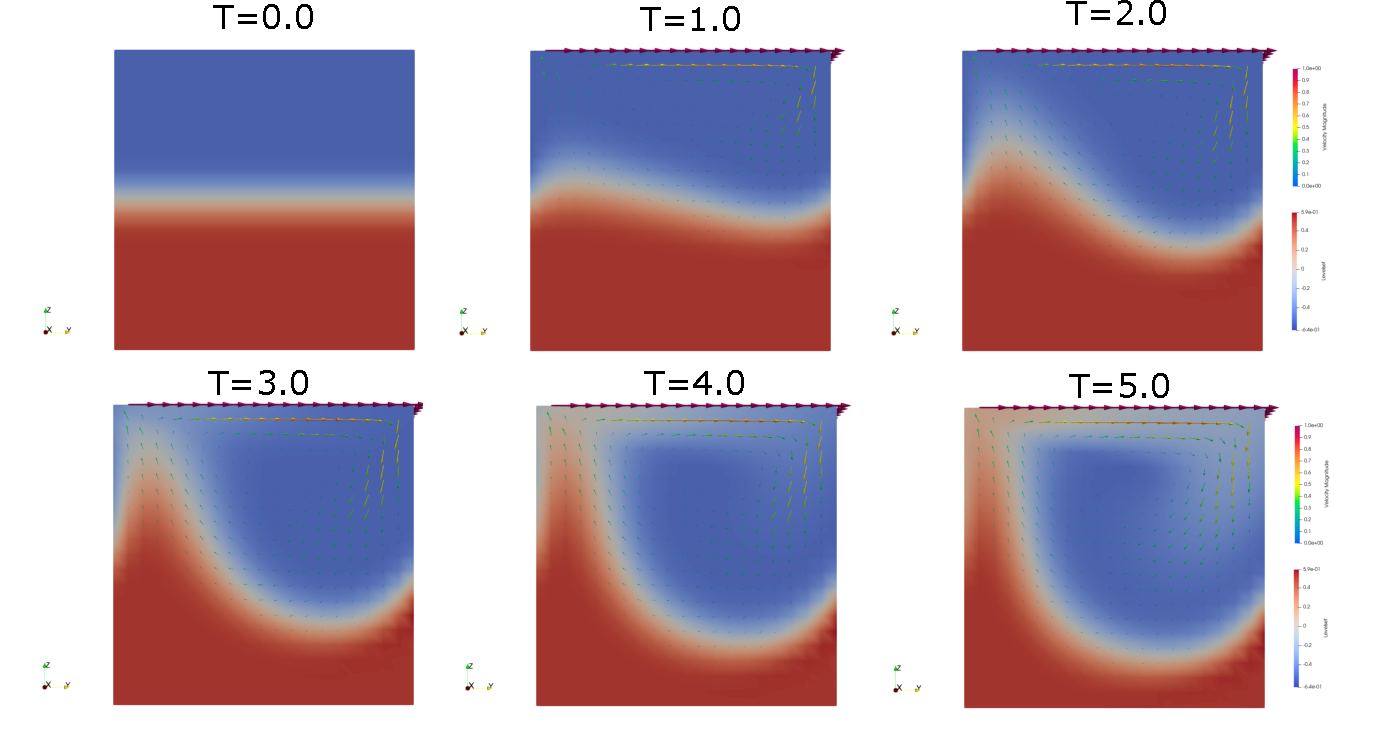
\includegraphics[width=18truecm]{pics/3d-cavity/levelset_velocity.pdf}
	\caption{二層キャビティ流れのレベルセット関数の時間変化($x=0.5$における断面)}
	\label{fig:3d-cavity-result-levelset}
\end{figure}

Figure \ref{fig:3d-cavity-result-velocity-pressure}に流速と圧力分布の結果を示す。
\begin{figure}[H]
	\centering
	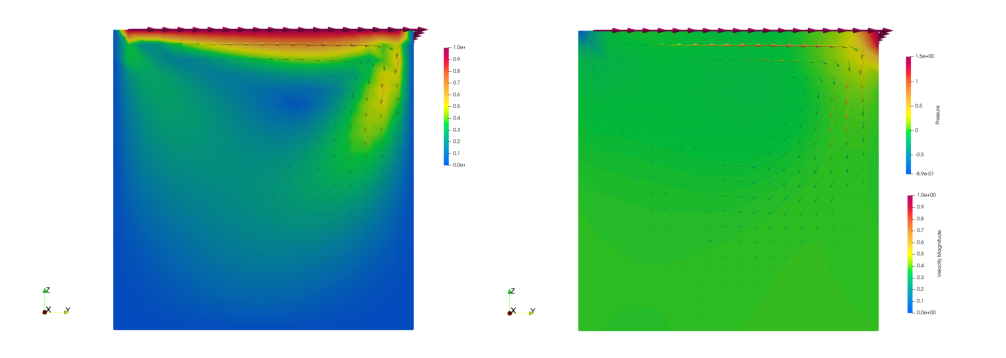
\includegraphics[width=18truecm]{pics/3d-cavity/velocity_pressure.pdf}
	\caption{二層キャビティ流れの速度と圧力分布($x=0.5$における断面)}
	\label{fig:3d-cavity-result-velocity-pressure}
\end{figure}

\begin{figure}[H]
	\centering
	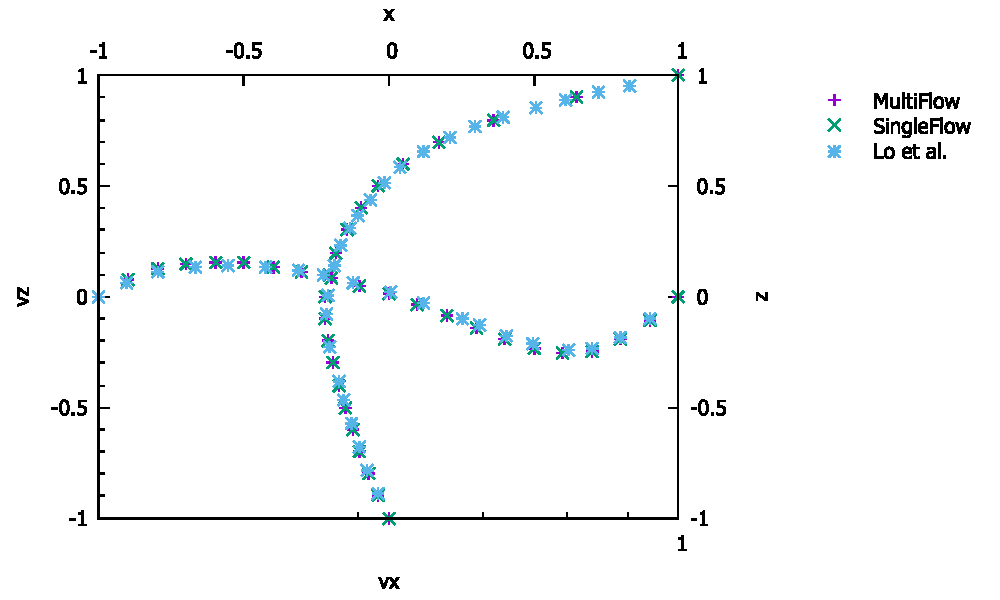
\includegraphics[width=18truecm]{pics/3d-cavity/velocity_graph.pdf}
	\caption{二層キャビティ流れと一層キャビティ流れの速度分布の比較によるプログラム検証$(T=30.0)$}
	\label{fig:3d-cavity_velocity_graph}
\end{figure}

Figure \ref{fig:3d-cavity_velocity_graph}より、単層流の場合と二層流の場合で速度分布が一致しており、また参考文献\cite{Lo2005}の結果ともよく一致しているため、プログラムの妥当性を検証できた。
\newpage
\section{3次元のダムブレイク問題}
二層流のベンチマーク問題として3次元のダムブレイク問題を解析した。

\subsection{解析条件}

Table \ref{table:dambreak-material-property}に二つの流体の物性値を示す。
Case1は水と空気の物性値である。
\renewcommand{\arraystretch}{1}
\begin{table}[H]
	\centering
	\caption{物性値}
	\begin{tabular}{ccccccc}
		\hline
		Test case & $\rho_1 (\mathrm{kg/m^3})$ & $\rho_2 (\mathrm{kg/m^3})$ & $\mu_1 (\mathrm{Ns/m^2})$& $\mu_2 (\mathrm{Ns/m^2})$ & $\mathrm{g} (\mathrm{m/s^2})$ \\
		\hline 
		Case$1$ & $998$ & $1.205$   & $1.01\times10^{-3}$ & $1.81\times10^{-5}$ & $9.81$ \\
		\hline         
	\end{tabular}
	\label{table:dambreak-material-property}
\end{table}
\renewcommand{\arraystretch}{1.0}

代表長さ$a=0.146 \mathrm{m}$として、
水柱の初期高さ$a(=0.146\mathrm{m})$、初期幅$2a(=0.292\mathrm{m})$、領域の高さ$2.4a(=0.3504\mathrm{m})$、幅$4a(=0.584\mathrm{m})$、奥行き$0.1a(=0.0146\mathrm{m})$とした。

Table \ref{table:dambreak-parameter}に解析における設定パラメータを示す。
界面幅$D$は、近似ヘビサイド関数よる平滑化の計算式(\ref{ls-heaviside})に含まれるパラメータである。
Case1と2では$D$の値が異なり、Case2の方がCase1よりも界面が平滑化される。
\renewcommand{\arraystretch}{1}
\begin{table}[H]
	\centering
	\caption{解析パラメータ}
	\begin{tabular}{cccccc}
		\hline
		Test case & $\Delta t$ & メッシュ幅$dx$ & 界面幅$D$ & 再初期化回数 & 再初期化$\Delta \tau$\\
		\hline 
		Case$1$ & $0.0001$ & $0.05$ & $0.05$ & $5$ & $0.01$\\
		\hline         
	\end{tabular}
	\label{table:dambreak-parameter}
\end{table}
\renewcommand{\arraystretch}{1.0}

Figure \ref{fig:3d-dambreak-mesh}に解析用のメッシュを示す。メッシュは六面体$1$次要素を使用した。
\begin{figure}[H]
	\centering
	\includegraphics[width=18truecm]{pics/3d-dambreak/mesh.pdf}
	\caption{ダムブレイクの計算メッシュ}
	\label{fig:3d-dambreak-mesh}
\end{figure}

Figure \ref{fig:3d-dambreak-boundary}に初期状態のレベルセット関数と、境界条件を示す。

\begin{figure}[H]
	\centering
	\includegraphics[width=18truecm]{pics/3d-dambreak/levelset_init.pdf}
	\caption{ダムブレイクの初期のレベルセット関数と境界条件}
	\label{fig:3d-dambreak-boundary}
\end{figure}

\subsection{解析結果}

\begin{figure}[H]
	\centering
	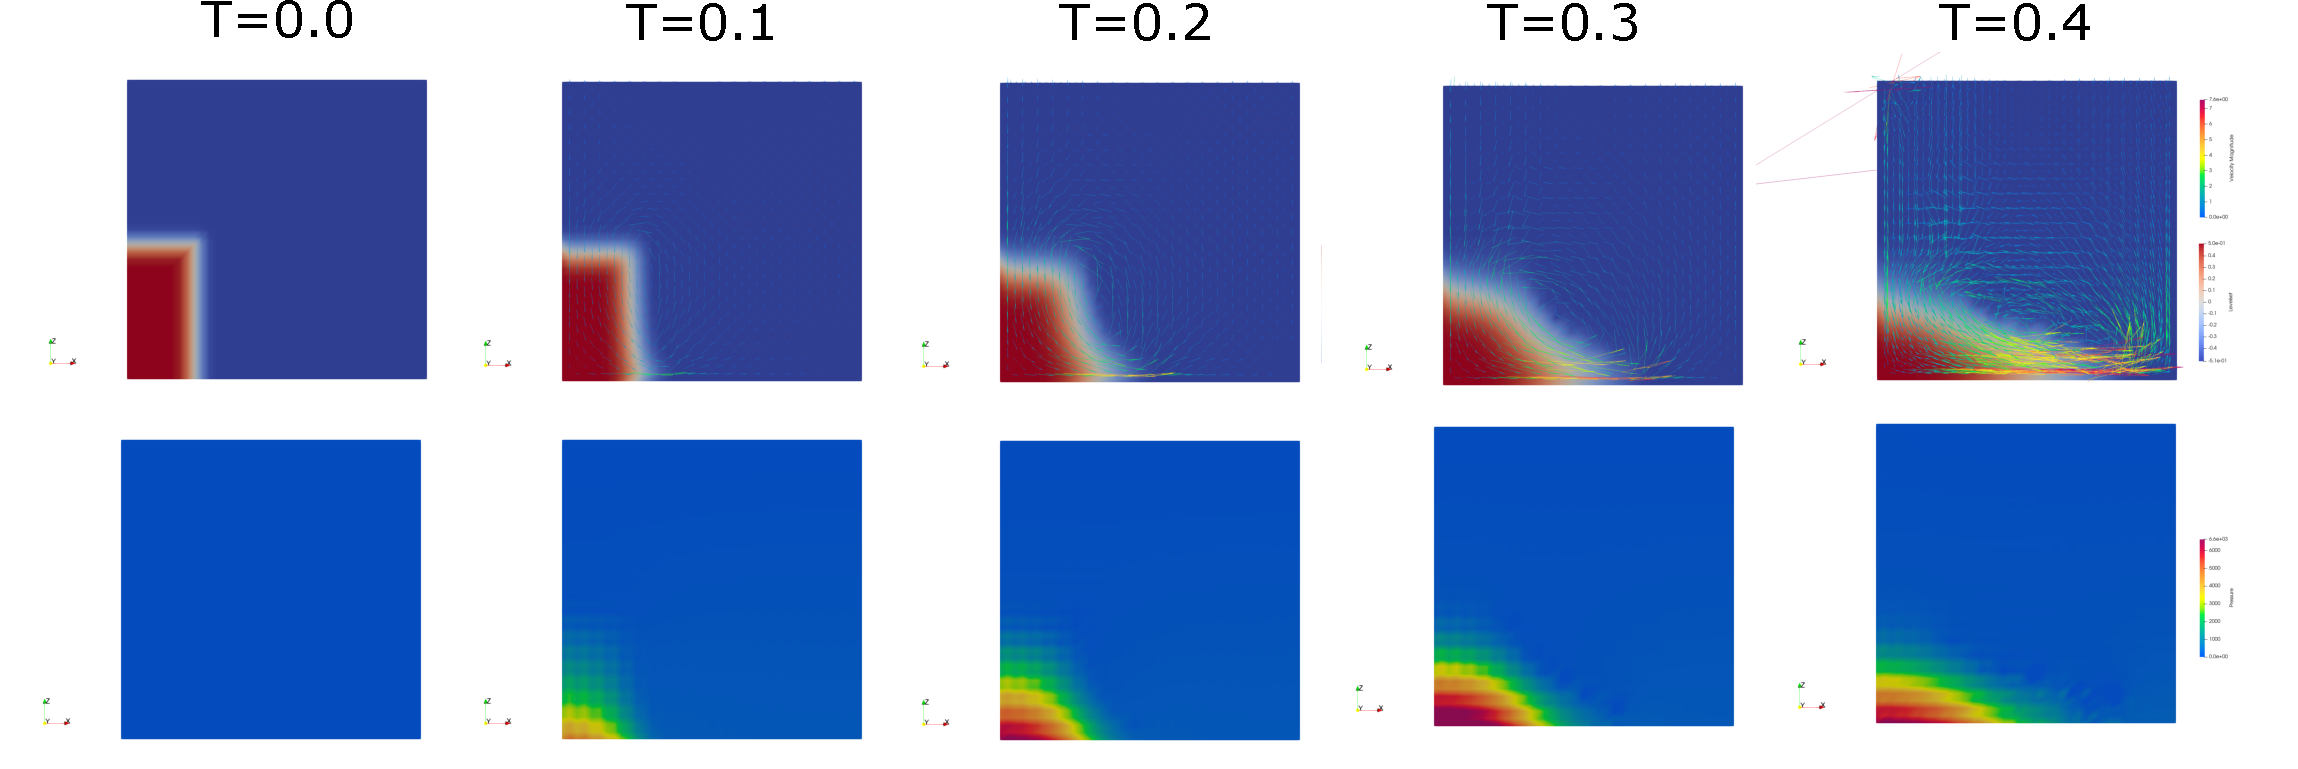
\includegraphics[width=18truecm]{pics/3d-dambreak/levelset_velocity.pdf}
	\caption{ダムブレイク問題の計算結果における速度と圧力分布}
	\label{fig:3d-dambreak-result}
\end{figure}

検証比較\cite{Martin1952}

\subsection{並列解析結果}
本ソルバーは領域分割法によるMPI並列化にも対応しているため、
3.5項で示した並列化解析実行手順に従い並列数を4として並列解析をした結果を示す。
Figure \ref{fig:3d-dambreak-parallel-partition}に領域分割したメッシュを示す。

\begin{figure}[H]
	\centering
	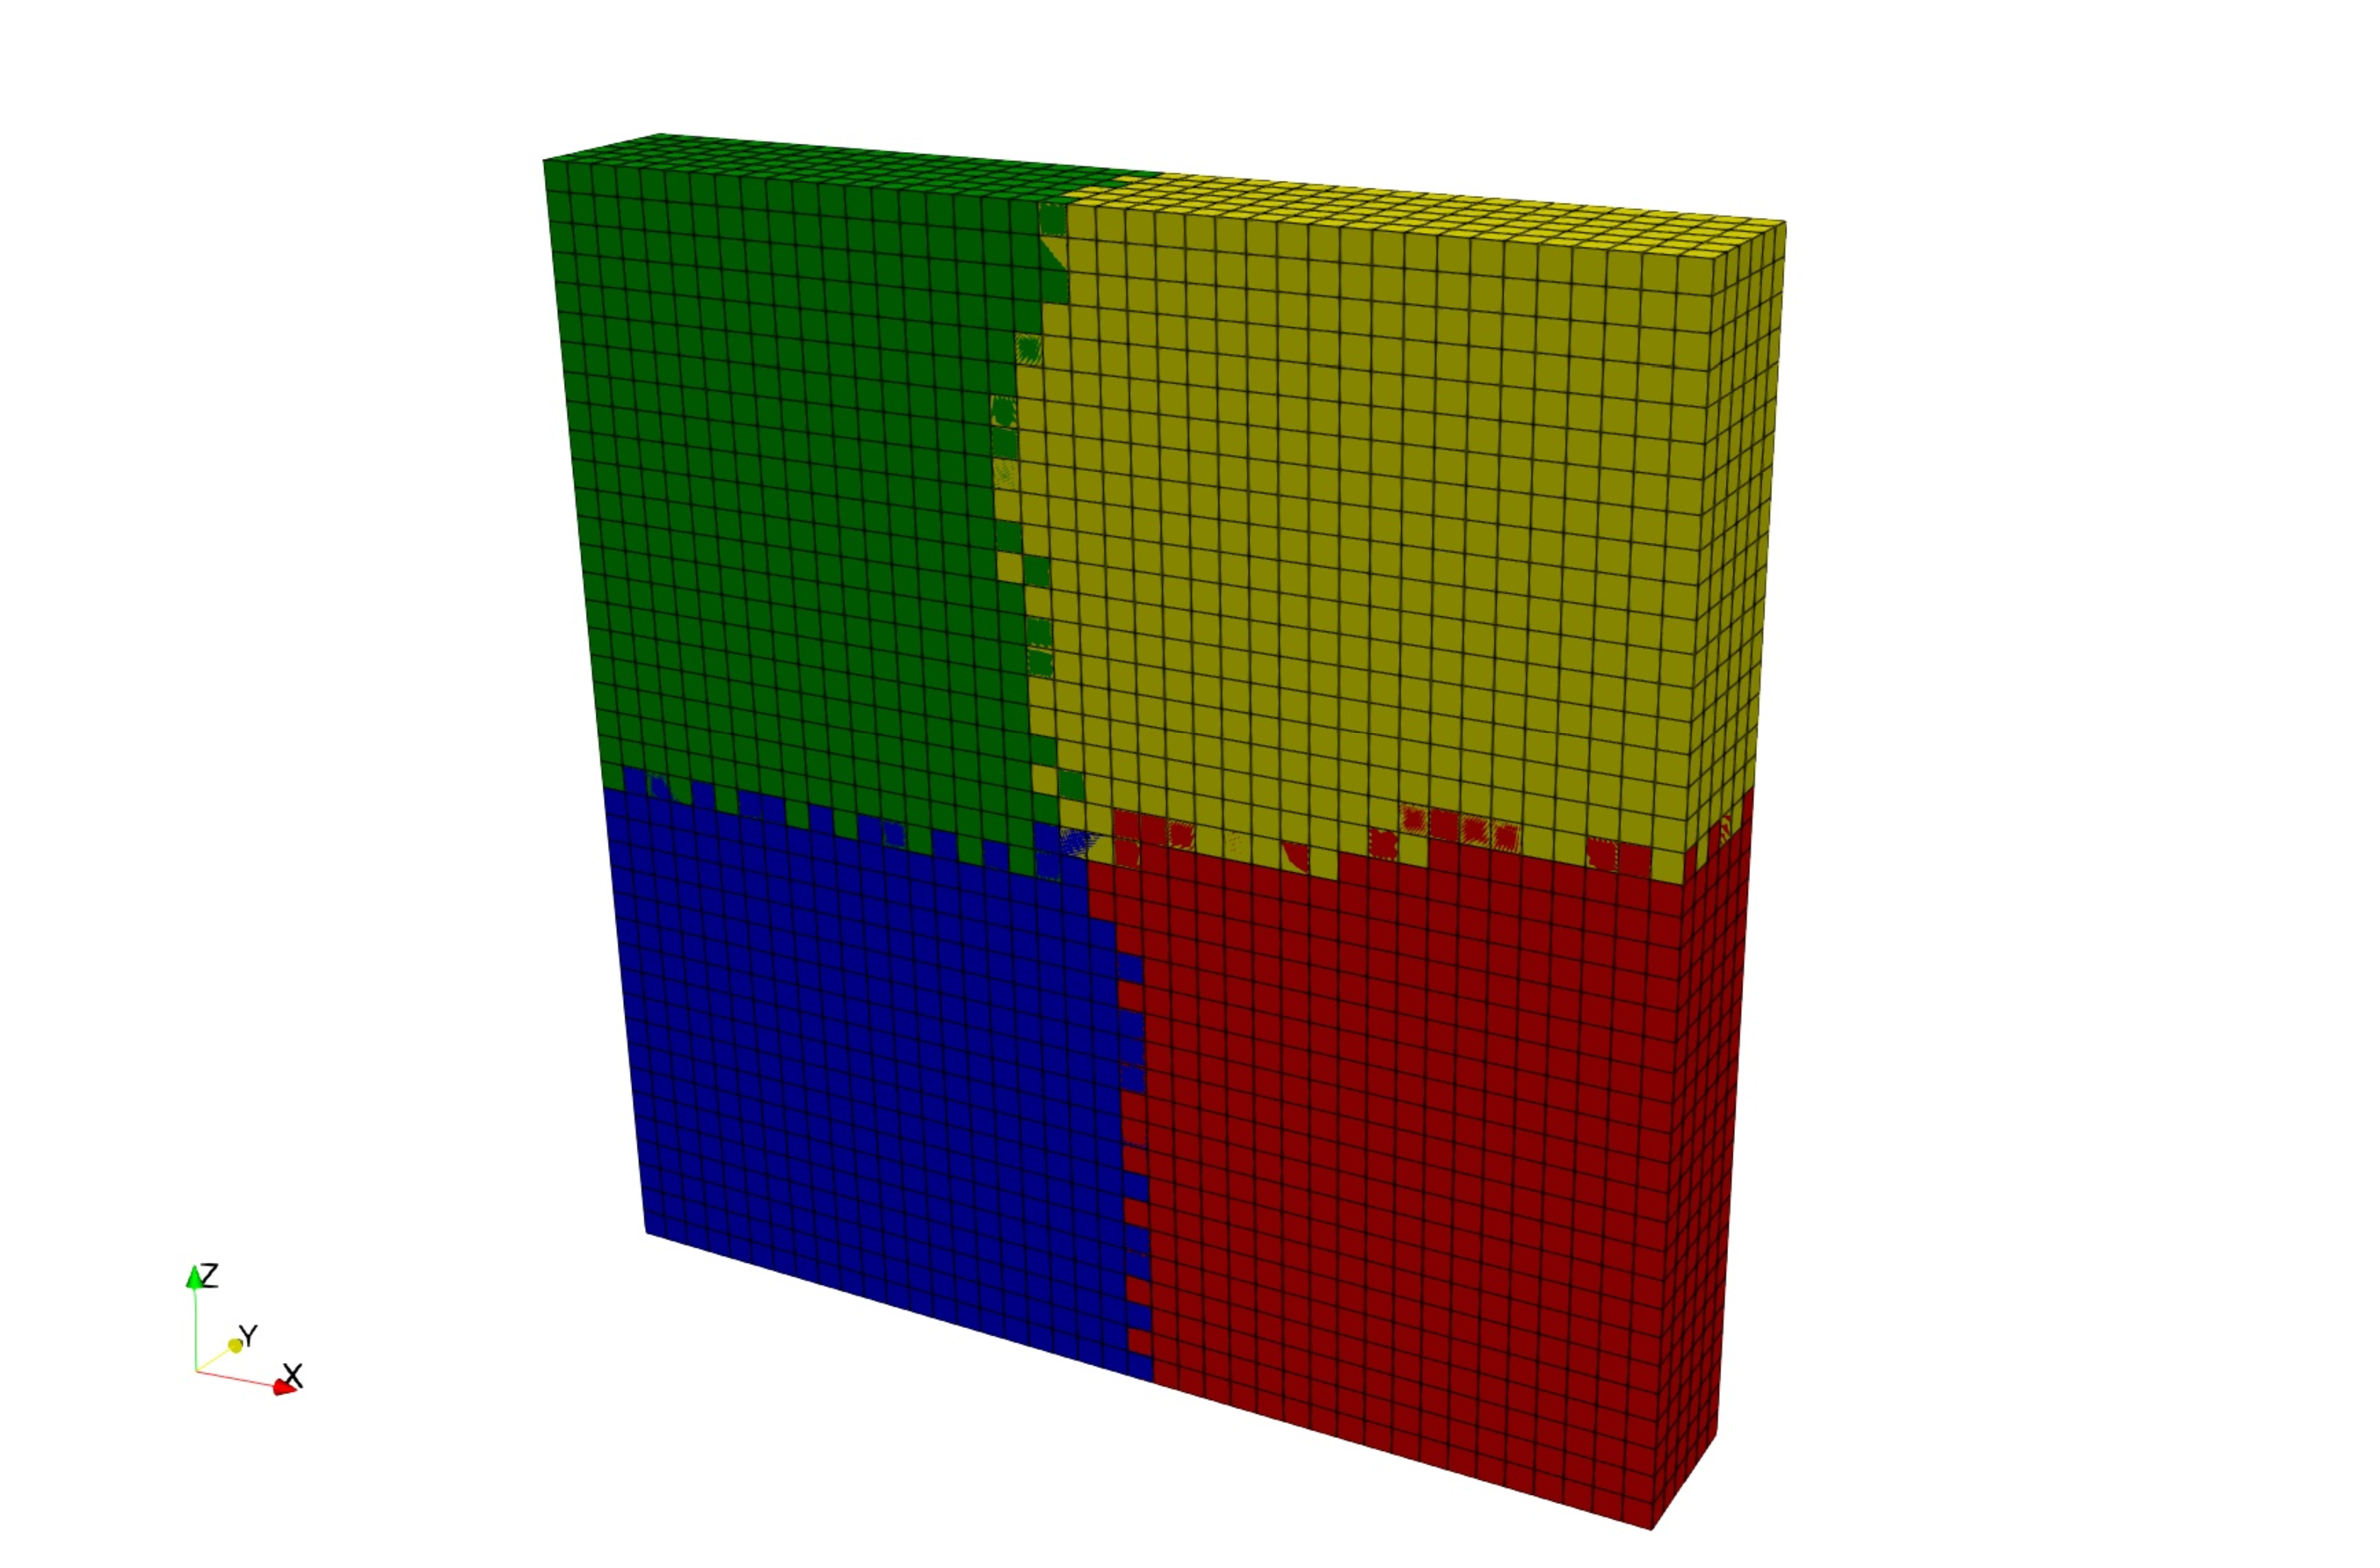
\includegraphics[width=18truecm]{pics/3d-dambreak-parallel/partition4.pdf}
	\caption{並列数4の場合の領域分割の図}
	\label{fig:3d-dambreak-parallel-partition}
\end{figure}

Figure \ref{fig:3d-dambreak-parallel-result}に速度分布、圧力分布、レベルセット関数の結果を示す。
並列化なしの場合と同様の結果が得られており、並列化解析が問題なくできていることが確認できた。
計算時間についても大幅に短くなっているが、時間計測は今回は行っていないため、今後スケーリング効果の計測を実施する。

\begin{figure}[H]
	\centering
	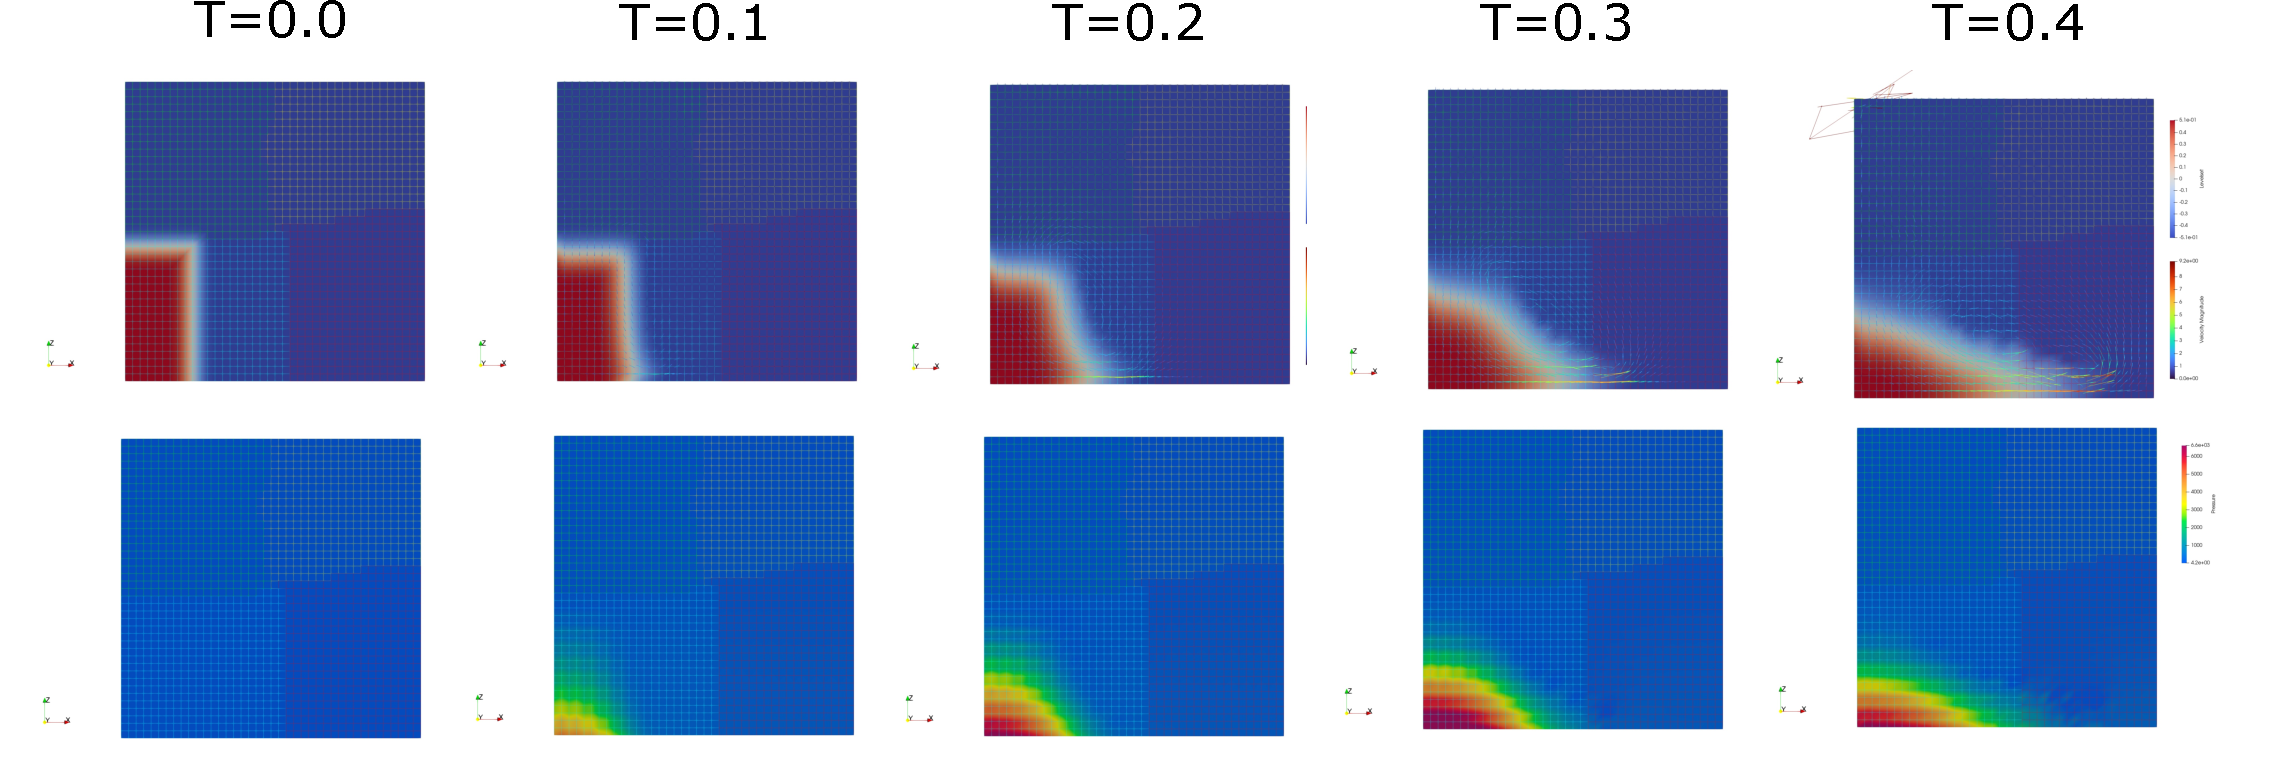
\includegraphics[width=18truecm]{pics/3d-dambreak-parallel/result-partition4.pdf}
	\caption{ダムブレイク問題のCase2の並列化解析による計算結果($y=0.4$における断面)。網目の色の違いで領域分割されている領域を可視化した。}
	\label{fig:3d-dambreak-parallel-result}
\end{figure}

ダムブレイクの検証\cite{Okumura2009}, 
有名な文献\cite{Koshizuka1996}

\newpage
\section{3次元気泡上昇流れ}

二層流の別のベンチマーク問題として3次元の気泡上昇流れ問題を解析し、参考文献の結果と比較した。

\subsection{解析条件}

Table \ref{table:3d-bubble-material-property}に二つの流体の物性値、Table \ref{table:3d-bubble-parameter}に解析パラメータを示す。
Case1は表面張力の影響が大きいケースであり、Case2は粘性の影響が大きいケースである。
ReとEoの値によって気泡の形が変わる分布を実験で分類している論文があり、Case1は球に近い形状を保った楕円形状であり、Case2では変形が大きくなる。

エトベス数$Eo = \rho g d^2 / \sigma$は、表面張力に対する重力の強さの指標。
ここで$d$は代表長さで気泡直径。(ボンド数Boとエトベス数Eoは同じ)


%ウェーバー数$We = \rho L U^2 / \sigma$は表面張力に対する慣性力の指標。
%\begin{figure}[H]
%	\centering
%	\includegraphics[width=6truecm]{pics/nond_number.png}
%	\caption{\cite{Himeno2023}}
%	\label{fig:3d-bubble-setting}
%\end{figure}

\renewcommand{\arraystretch}{1}
\begin{table}[H]
	\centering
	\caption{物性値}
	\begin{tabular}{cccccccccc}
		\hline
		Test case & $\rho_1$ & $\rho_2$ & $\mu_1$ & $\mu_2$ & $\mathrm{g}$ & $\sigma$ & $Eo (Bo)$ & $Re$ \\
		\hline 
		Case$1$ & $1000$ & $100$ & $10$ & $1$   & $0.98$ & $24.5$ & $10$ & $35$\\
		Case$2$ & $1000$ & $1$   & $10$ & $0.1$ & $0.98$ & $1.96$ & $125$ & $35$\\ 
		\hline         
	\end{tabular}
	\label{table:3d-bubble-material-property}
\end{table}
\renewcommand{\arraystretch}{1.0}

Case1は表面張力が強いため、数値安定性のために$\tau$を小さくする必要がある。\cite{Yamaguchi2018}
%表面張力の時間刻み制約は$\Delta t_{s} = \sqrt{(1000 + 100)\cdot \frac{10}{8 \pi}}\cdot 0.05^{\frac{3}{2}} = 0.234$

\renewcommand{\arraystretch}{1}
\begin{table}[H]
	\centering
	\caption{解析パラメータ}
	\begin{tabular}{cccccc}
		\hline
		Test case & $\Delta t$ & メッシュ幅$dx$ & 界面幅$D$ & 再初期化回数 & 再初期化$\Delta \tau$\\
		\hline 
		Case$1$ & $0.0025$ & $0.05$ & $0.04$ & $5$ & $0.001$\\
		Case$2$ & $0.0025$ & $0.05$ & $0.04$ & $5$ & $0.001$\\
		\hline         
	\end{tabular}
	\label{table:3d-bubble-parameter}
\end{table}
\renewcommand{\arraystretch}{1.0}

Figure \ref{fig:3d-bubble-setting}に文献\cite{Safi2017}から引用した解析領域の図を示す。

\begin{figure}[H]
	\centering
	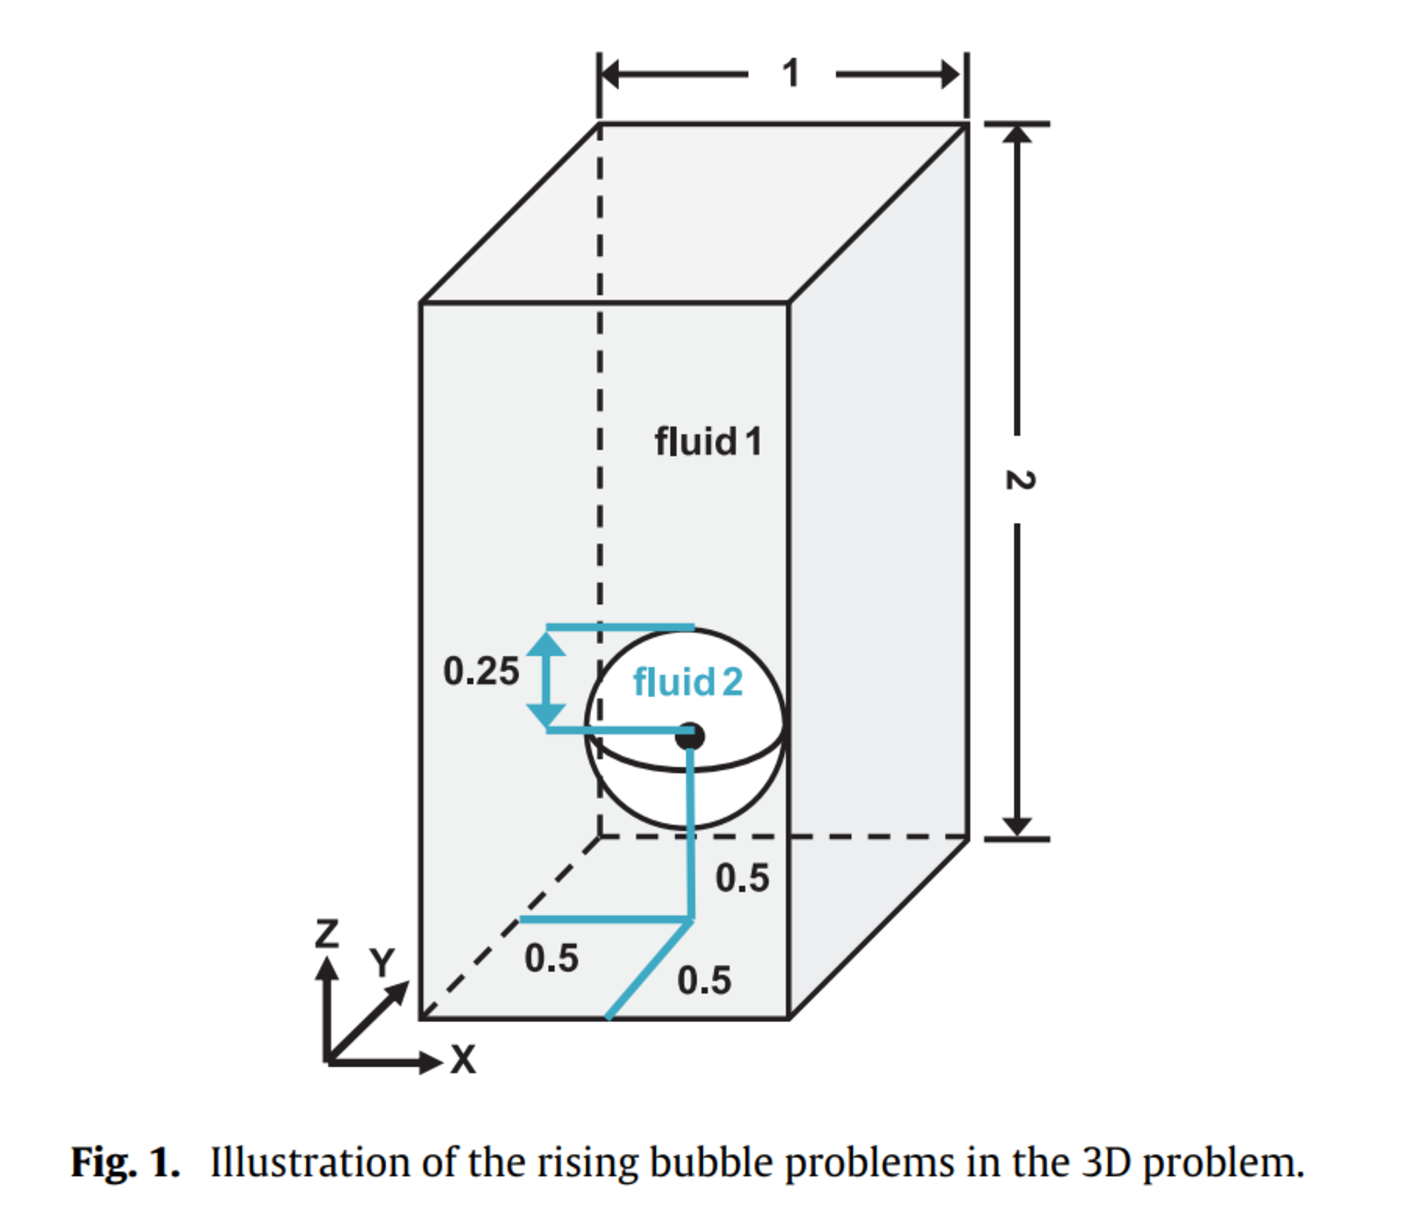
\includegraphics[width=10truecm]{pics/3d-bubble/setting.pdf}
	\caption{解析条件\cite{Safi2017}}
	\label{fig:3d-bubble-setting}
\end{figure}

Figure \ref{fig:3d-bubble-mesh}に解析用のメッシュを示す。メッシュは四面体$1$次要素を使用した。境界条件はダムブレイク問題と同様に上面を流出境界条件として圧力のディリクレ境界条件$p=0$、それ以外の面を滑りなし壁境界とした。
Figure \ref{fig:3d-bubble-levelset_t0_3d}に初期状態のレベルセット関数を示す。白い球面が界面である。

\begin{figure}[H]
	\centering
	\begin{minipage}[b]{0.49\columnwidth}
	    \centering
	    \includegraphics[width=6truecm]{pics/3d-bubble/mesh.jpeg}
		\caption{3次元気泡上昇流れの計算メッシュ}
		\label{fig:3d-bubble-mesh}
	\end{minipage}
	\begin{minipage}[b]{0.49\columnwidth}
	    \centering
	    \includegraphics[width=6truecm]{pics/3d-bubble/levelset_init.jpeg}
		\caption{3次元気泡上昇流れのレベルセット関数($T=0$)}
		\label{fig:3d-bubble-levelset_t0_3d}
	\end{minipage}
\end{figure}

\newpage
\subsection{解析結果(Case1, 表面張力の影響が大きいケース)}
気泡上昇流れ問題においては表面張力の影響は大きいと思われるため、表面張力のモデルを導入し計算した結果を示す。

\begin{figure}[H]
	\centering
	\begin{minipage}[b]{0.16\columnwidth}
	    \centering
	    \includegraphics[width=3.3truecm]{pics/3d-bubble/tc1/result_0005.jpeg}
	\end{minipage}
	\begin{minipage}[b]{0.16\columnwidth}
	    \centering
	    \includegraphics[width=3.3truecm]{pics/3d-bubble/tc1/result_0015.jpeg}
	\end{minipage}
	\begin{minipage}[b]{0.16\columnwidth}
	    \centering
	    \includegraphics[width=3.3truecm]{pics/3d-bubble/tc1/result_0020.jpeg}
	\end{minipage}
	\begin{minipage}[b]{0.16\columnwidth}
	    \centering
	    \includegraphics[width=3.3truecm]{pics/3d-bubble/tc1/result_0025.jpeg}
	\end{minipage}
	\begin{minipage}[b]{0.16\columnwidth}
	    \centering
	    \includegraphics[width=3.3truecm]{pics/3d-bubble/tc1/result_0030.jpeg}
	\end{minipage}

	\caption{3次元気泡上昇流れのレベルセット関数の分布の時間変化(Case1, $\sigma=24.5$、表面張力あり、体積保存あり、再初期化あり)}
	\label{fig:3d-bubble_result_tc1}
\end{figure}

\begin{figure}[H]
    \centering
	\includegraphics[width=15truecm]{pics/3d-bubble/result-ref-tc1.png}
	\caption{参考文献結果(Case1)\cite{Safi2017}}
	\label{fig:3d-bubble-result-ref}
\end{figure}

\begin{figure}[H]
	\centering
	\begin{minipage}[b]{0.49\columnwidth}
	    \centering
	    \includegraphics[width=8truecm]{pics/3d-bubble/tc1_center.pdf}
		\caption{重心位置の時間変化(Case1)}
		\label{fig:3d-bubble-center-tc1}
	\end{minipage}
	\begin{minipage}[b]{0.49\columnwidth}
	    \centering
	    \includegraphics[width=8truecm]{pics/3d-bubble/tc1_velocity.pdf}
		\caption{上昇速度の時間変化(Case1)}
		\label{fig:3d-bubble-velocity-tc1}
	\end{minipage}
\end{figure}


\subsubsection{表面張力なしの解析結果}
\begin{figure}[H]
	\centering
	\begin{minipage}[b]{0.16\columnwidth}
	    \centering
	    \includegraphics[width=3.3truecm]{pics/3d-bubble/tc1-nosurfacetension/result_0005.jpeg}
	\end{minipage}
	\begin{minipage}[b]{0.16\columnwidth}
	    \centering
	    \includegraphics[width=3.3truecm]{pics/3d-bubble/tc1-nosurfacetension/result_0015.jpeg}
	\end{minipage}
	\begin{minipage}[b]{0.16\columnwidth}
	    \centering
	    \includegraphics[width=3.3truecm]{pics/3d-bubble/tc1-nosurfacetension/result_0020.jpeg}
	\end{minipage}
	\begin{minipage}[b]{0.16\columnwidth}
	    \centering
	    \includegraphics[width=3.3truecm]{pics/3d-bubble/tc1-nosurfacetension/result_0025.jpeg}
	\end{minipage}
	\begin{minipage}[b]{0.16\columnwidth}
	    \centering
	    \includegraphics[width=3.3truecm]{pics/3d-bubble/tc1-nosurfacetension/result_0029.jpeg}
	\end{minipage}

	\caption{3次元気泡上昇流れのレベルセット関数の分布の時間変化(Case1, $\sigma=0$、表面張力なし、体積保存あり、再初期化あり)}
	\label{fig:3d-bubble_result_tc1}
\end{figure}

\subsubsection{体積保存なしの解析結果}
\begin{figure}[H]
	\centering
	\begin{minipage}[b]{0.16\columnwidth}
	    \centering
	    \includegraphics[width=3.3truecm]{pics/3d-bubble/tc1-novolumecorrection/result_0005.jpeg}
	\end{minipage}
	\begin{minipage}[b]{0.16\columnwidth}
	    \centering
	    \includegraphics[width=3.3truecm]{pics/3d-bubble/tc1-novolumecorrection/result_0015.jpeg}
	\end{minipage}
	\begin{minipage}[b]{0.16\columnwidth}
	    \centering
	    \includegraphics[width=3.3truecm]{pics/3d-bubble/tc1-novolumecorrection/result_0020.jpeg}
	\end{minipage}
	\begin{minipage}[b]{0.16\columnwidth}
	    \centering
	    \includegraphics[width=3.3truecm]{pics/3d-bubble/tc1-novolumecorrection/result_0025.jpeg}
	\end{minipage}
	\begin{minipage}[b]{0.16\columnwidth}
	    \centering
	    \includegraphics[width=3.3truecm]{pics/3d-bubble/tc1-novolumecorrection/result_0030.jpeg}
	\end{minipage}

	\caption{3次元気泡上昇流れのレベルセット関数の分布の時間変化(Case1, $\sigma=24.5$、表面張力あり、体積保存なし、再初期化あり)}
	\label{fig:3d-bubble_result_tc1}
\end{figure}

\subsubsection{再初期化なしの解析結果}
\begin{figure}[H]
	\centering
	\begin{minipage}[b]{0.16\columnwidth}
	    \centering
	    \includegraphics[width=3.3truecm]{pics/3d-bubble/tc1-noreinitialization/result_0002.jpeg}
	\end{minipage}
	\begin{minipage}[b]{0.16\columnwidth}
	    \centering
	    \includegraphics[width=3.3truecm]{pics/3d-bubble/tc1-noreinitialization/result_0004.jpeg}
	\end{minipage}
	\begin{minipage}[b]{0.16\columnwidth}
	    \centering
	    \includegraphics[width=3.3truecm]{pics/3d-bubble/tc1-noreinitialization/result_0006.jpeg}
	\end{minipage}
	\begin{minipage}[b]{0.16\columnwidth}
	    \centering
	    \includegraphics[width=3.3truecm]{pics/3d-bubble/tc1-noreinitialization/result_0008.jpeg}
	\end{minipage}
	\begin{minipage}[b]{0.16\columnwidth}
	    \centering
	    \includegraphics[width=3.3truecm]{pics/3d-bubble/tc1-noreinitialization/result_0010.jpeg}
	\end{minipage}

	\caption{3次元気泡上昇流れのレベルセット関数の分布の時間変化(Case1, $\sigma=24.5$、表面張力あり、体積保存あり、再初期化なし)}
	\label{fig:3d-bubble_result_tc1}
\end{figure}

\newpage
\subsection{解析結果(Case2, 表面張力の影響が小さいケース)}
\begin{figure}[H]
	\centering
	\begin{minipage}[b]{0.16\columnwidth}
	    \centering
	    \includegraphics[width=3.3truecm]{pics/3d-bubble/tc2/result_0005.jpeg}
	\end{minipage}
	\begin{minipage}[b]{0.16\columnwidth}
	    \centering
	    \includegraphics[width=3.3truecm]{pics/3d-bubble/tc2/result_0015.jpeg}
	\end{minipage}
	\begin{minipage}[b]{0.16\columnwidth}
	    \centering
	    \includegraphics[width=3.3truecm]{pics/3d-bubble/tc2/result_0020.jpeg}
	\end{minipage}
	\begin{minipage}[b]{0.16\columnwidth}
	    \centering
	    \includegraphics[width=3.3truecm]{pics/3d-bubble/tc2/result_0025.jpeg}
	\end{minipage}
	\begin{minipage}[b]{0.16\columnwidth}
	    \centering
	    \includegraphics[width=3.3truecm]{pics/3d-bubble/tc2/result_0030.jpeg}
	\end{minipage}

	\caption{3次元気泡上昇流れのレベルセット関数の分布の時間変化(Case2, $\sigma=1.95$、表面張力あり)}
	\label{fig:3d-bubble_result_tc2}
\end{figure}

\begin{figure}[H]
	\centering
	\begin{minipage}[b]{0.16\columnwidth}
	    \centering
	    \includegraphics[width=3.3truecm]{pics/3d-bubble/tc2-d010/result_0005.jpeg}
	\end{minipage}
	\begin{minipage}[b]{0.16\columnwidth}
	    \centering
	    \includegraphics[width=3.3truecm]{pics/3d-bubble/tc2-d010/result_0015.jpeg}
	\end{minipage}
	\begin{minipage}[b]{0.16\columnwidth}
	    \centering
	    \includegraphics[width=3.3truecm]{pics/3d-bubble/tc2-d010/result_0020.jpeg}
	\end{minipage}
	\begin{minipage}[b]{0.16\columnwidth}
	    \centering
	    \includegraphics[width=3.3truecm]{pics/3d-bubble/tc2-d010/result_0025.jpeg}
	\end{minipage}
	\begin{minipage}[b]{0.16\columnwidth}
	    \centering
	    \includegraphics[width=3.3truecm]{pics/3d-bubble/tc2-d010/result_0030.jpeg}
	\end{minipage}

	\caption{3次元気泡上昇流れのレベルセット関数の分布の時間変化(Case2, $\sigma=1.95$、表面張力あり、界面幅$D=0.10$)}
	\label{fig:3d-bubble_result_tc2}
\end{figure}

\begin{figure}[H]
    \centering
	\includegraphics[width=15truecm]{pics/3d-bubble/result-ref-tc2.png}
	\caption{参考文献結果(Case2)\cite{Safi2017}}
	\label{fig:3d-bubble-result-ref}
\end{figure}

\begin{figure}[H]
	\centering
	\begin{minipage}[b]{0.49\columnwidth}
	    \centering
	    \includegraphics[width=8truecm]{pics/3d-bubble/tc2_center.pdf}
		\caption{重心位置の時間変化(Case2)}
		\label{fig:3d-bubble-center-tc2}
	\end{minipage}
	\begin{minipage}[b]{0.49\columnwidth}
	    \centering
	    \includegraphics[width=8truecm]{pics/3d-bubble/tc2_velocity.pdf}
		\caption{上昇速度の時間変化(Case2)}
		\label{fig:3d-bubble-velocity-tc2}
	\end{minipage}
\end{figure}

\newpage
\section{3次元スロッシング}

数値解析例として矩形緒層内スロッシング解析を実施し、参考文献の結果と比較した。

\subsection{解析条件}

物性値パラメータを表\ref{table:3d-sloshing-material-property}に示す。流体は水と空気を仮定したパラメータである。
\renewcommand{\arraystretch}{1}
\begin{table}[H]
	\centering
	\caption{物性値}
	\begin{tabular}{ccccccc}
		\hline
		Test case & $\rho_1$ & $\rho_2$ & $\mu_1$ & $\mu_2$ & $\mathrm{g}$ \\
		\hline 
		Case$1$ & $1000$ & $1.2$ & $1.0e-3$ & $1.8e-5$ & $9.8$ \\
		\hline         
	\end{tabular}
	\label{table:3d-sloshing-material-property}
\end{table}
\renewcommand{\arraystretch}{1.0}

解析パラメータを表\ref{table:3d-sloshing-parameter}に示す。メッシュの細かさの違う条件で解析し、精度検証した。
\renewcommand{\arraystretch}{1}
\begin{table}[H]
	\centering
	\caption{解析パラメータ}
	\begin{tabular}{cccccc}
		\hline
		Test case & $\Delta t$ & メッシュ幅$dx$ & 界面幅$D$ & 再初期化回数 & 再初期化$\Delta \tau$\\
		\hline 
		Case$1$ & $0.0025$ & $0.025$ & $0.075$ & $5$ & $0.0001$\\
		Case$2$ & $0.0010$ & $0.0125$ & $0.030$ & $5$ & $0.0001$\\
		\hline         
	\end{tabular}
	\label{table:3d-sloshing-parameter}
\end{table}
\renewcommand{\arraystretch}{1.0}

解析領域は幅$1.0\mathrm{m}$、奥行き$0.2\mathrm{m}$、高さ$1.2\mathrm{m}$であり、水が高さ$0.5\mathrm{m}$まで入っている状態である。
境界条件は全壁面でスリップ条件を与えた。
メッシュは六面体1次要素で、節点数18,081、要素数15,360である。

\begin{figure}[H]
	\centering
	\begin{minipage}[b]{0.49\columnwidth}
	    \centering
	    \includegraphics[width=6truecm]{pics/3d-sloshing/mesh.jpeg}
		\caption{3次元スロッシングの計算メッシュ}
		\label{fig:3d-sloshing-mesh}
	\end{minipage}
	\begin{minipage}[b]{0.49\columnwidth}
	    \centering
	    \includegraphics[width=6truecm]{pics/3d-sloshing/levelset_init.jpeg}
		\caption{3次元スロッシングのレベルセット関数($T=0$)}
		\label{fig:3d-sloshing-levelset_t0_3d}
	\end{minipage}
\end{figure}

スロッシングを起こすための水平加速度$f_{x}$は以下の式で与える。
\begin{equation}
	f_{x} = A \omega^2 \sin{\omega t}
\end{equation}
ここで、振幅$A=0.0093 \mathrm{m}$、角速度$\omega = 5.311 \mathrm{rad/s}$と設定した。

\newpage
\subsection{解析結果}
\subsubsection{メッシュ固定の場合の解析結果}

\begin{figure}[H]
	\centering
	\begin{minipage}[b]{0.19\columnwidth}
	    \centering
	    \includegraphics[width=3.5truecm]{pics/3d-sloshing/CN-dx0025/result_0010.jpeg}
	\end{minipage}
	\begin{minipage}[b]{0.19\columnwidth}
	    \centering
	    \includegraphics[width=3.5truecm]{pics/3d-sloshing/CN-dx0025/result_0012.jpeg}
	\end{minipage}
	\begin{minipage}[b]{0.19\columnwidth}
	    \centering
	    \includegraphics[width=3.5truecm]{pics/3d-sloshing/CN-dx0025/result_0014.jpeg}
	\end{minipage}
	\begin{minipage}[b]{0.19\columnwidth}
	    \centering
	    \includegraphics[width=3.5truecm]{pics/3d-sloshing/CN-dx0025/result_0016.jpeg}
	\end{minipage}
	\begin{minipage}[b]{0.19\columnwidth}
	    \centering
	    \includegraphics[width=3.5truecm]{pics/3d-sloshing/CN-dx0025/result_0018.jpeg}
	\end{minipage}
	\caption{スロッシングの結果($1.0\mathrm{s}$~$1.8\mathrm{s}$)}
	\label{fig:sloshing-result}
\end{figure}
\begin{figure}[H]
	\centering
	\begin{minipage}[b]{0.19\columnwidth}
	    \centering
	    \includegraphics[width=3.5truecm]{pics/3d-sloshing/CN-dx0025/result_0090.jpeg}
	\end{minipage}
	\begin{minipage}[b]{0.19\columnwidth}
	    \centering
	    \includegraphics[width=3.5truecm]{pics/3d-sloshing/CN-dx0025/result_0092.jpeg}
	\end{minipage}
	\begin{minipage}[b]{0.19\columnwidth}
	    \centering
	    \includegraphics[width=3.5truecm]{pics/3d-sloshing/CN-dx0025/result_0094.jpeg}
	\end{minipage}
	\begin{minipage}[b]{0.19\columnwidth}
	    \centering
	    \includegraphics[width=3.5truecm]{pics/3d-sloshing/CN-dx0025/result_0096.jpeg}
	\end{minipage}
	\begin{minipage}[b]{0.19\columnwidth}
	    \centering
	    \includegraphics[width=3.5truecm]{pics/3d-sloshing/CN-dx0025/result_0098.jpeg}
	\end{minipage}
	\caption{スロッシングの結果($9.0\mathrm{s}$~$9.8\mathrm{s}$)}
	\label{fig:sloshing-result}
\end{figure}

解析結果の左端の水位の時間変化のグラフを図~\ref{fig:3d-sloshing-result}に示す。
流体メッシュは固定して慣性加速度を与えた場合と、流体メッシュに加速度を与えて移動させた場合(ALE)の結果を比較し、どちらも近い結果が得られた。
さらにメッシュを粗いケースと細かいケースで計算したところ、細かくすることによって文献の値により近い結果が得られた。
\begin{figure}[H]
    \centering
	\includegraphics[width=15truecm]{pics/3d-sloshing/height_time.pdf}
	\caption{スロッシング解析結果の左端の水位と参考文献\cite{Okamoto1992}, \cite{Sakuraba2001}との比較}
	\label{fig:3d-sloshing-result}
\end{figure}

参考までに、スロッシング解析では衝撃捕捉項(\ref{sec:fluid}章の式(\ref{fluid-GLS}))を入れない場合、6.0sあたりから計算が不安定になり発散しやすい傾向が見られた。
実際にALE法ではあるが、shock capturing項(衝撃捕捉項)を入れない場合と入れる場合の計算を比較し、入れない場合は6.0s過ぎた付近から計算が不安定となり、その後発散するが、入れた場合は安定的に計算ができた結果が報告されている\cite{Sakuraba1999}。

\newpage
\subsubsection{メッシュを移動させた場合の解析結果(ALE記述の実装の確認)}
ここでは、メッシュを移動させた場合の結果を示す。

\begin{figure}[H]
	\centering
	\begin{minipage}[b]{0.19\columnwidth}
	    \centering
	    \includegraphics[width=3.5truecm]{pics/3d-sloshing/ALE-dx0025/result_0010.jpeg}
	\end{minipage}
	\begin{minipage}[b]{0.19\columnwidth}
	    \centering
	    \includegraphics[width=3.5truecm]{pics/3d-sloshing/ALE-dx0025/result_0012.jpeg}
	\end{minipage}
	\begin{minipage}[b]{0.19\columnwidth}
	    \centering
	    \includegraphics[width=3.5truecm]{pics/3d-sloshing/ALE-dx0025/result_0014.jpeg}
	\end{minipage}
	\begin{minipage}[b]{0.19\columnwidth}
	    \centering
	    \includegraphics[width=3.5truecm]{pics/3d-sloshing/ALE-dx0025/result_0016.jpeg}
	\end{minipage}
	\begin{minipage}[b]{0.19\columnwidth}
	    \centering
	    \includegraphics[width=3.5truecm]{pics/3d-sloshing/ALE-dx0025/result_0018.jpeg}
	\end{minipage}
	\caption{スロッシングの結果($1.0\mathrm{s}$~$1.8\mathrm{s}$)}
	\label{fig:sloshing-result}
\end{figure}
\begin{figure}[H]
	\centering
	\begin{minipage}[b]{0.19\columnwidth}
	    \centering
	    \includegraphics[width=3.5truecm]{pics/3d-sloshing/ALE-dx0025/result_0090.jpeg}
	\end{minipage}
	\begin{minipage}[b]{0.19\columnwidth}
	    \centering
	    \includegraphics[width=3.5truecm]{pics/3d-sloshing/ALE-dx0025/result_0092.jpeg}
	\end{minipage}
	\begin{minipage}[b]{0.19\columnwidth}
	    \centering
	    \includegraphics[width=3.5truecm]{pics/3d-sloshing/ALE-dx0025/result_0094.jpeg}
	\end{minipage}
	\begin{minipage}[b]{0.19\columnwidth}
	    \centering
	    \includegraphics[width=3.5truecm]{pics/3d-sloshing/ALE-dx0025/result_0096.jpeg}
	\end{minipage}
	\begin{minipage}[b]{0.19\columnwidth}
	    \centering
	    \includegraphics[width=3.5truecm]{pics/3d-sloshing/ALE-dx0025/result_0098.jpeg}
	\end{minipage}
	\caption{スロッシングの結果($9.0\mathrm{s}$~$9.8\mathrm{s}$)}
	\label{fig:sloshing-result}
\end{figure}

\newpage
\subsection{解析結果(並列化計算)}

領域分割法による並列計算結果についても検証を行った。
図~\ref{fig:3d-sloshing-mesh-parallel16}に領域分割数16の場合の計算メッシュの分割結果を示す。
節点数は23571, 要素数は15360である。

\begin{figure}[H]
    \centering
    \includegraphics[width=6truecm]{pics/3d-sloshing-parallel/mesh_parallel16.jpeg}
	\caption{スロッシングの計算メッシュ(領域分割数16の場合)}
	\label{fig:3d-sloshing-mesh-parallel16}
\end{figure}

図~\ref{fig:3d-sloshing-result-parallel}に並列数2,4, 8, 16の場合の計算結果を示す。
並列数を変えた場合でも逐次計算の結果と一致した結果が得られた。

\begin{figure}[H]
    \centering
	\includegraphics[width=15truecm]{pics/3d-sloshing-parallel/sloshing_result_comparison_parallel.pdf}
	\caption{スロッシング解析結果の左端の水位と参考文献\cite{Okamoto1992}, \cite{Sakuraba2001}との比較}
	\label{fig:3d-sloshing-result-parallel}
\end{figure}

図~\ref{fig:3d-sloshing-parallel-speedup}に並列化による加速率効率のグラフを示す。
\begin{figure}[H]
    \centering
	\includegraphics[width=15truecm]{pics/3d-sloshing-parallel/sloshing_parallel_speedup.jpg}
	\caption{スロッシング解析の並列化効率}
	\label{fig:3d-sloshing-parallel-speedup}
\end{figure}

\begin{thebibliography}{99}
	\bibitem{Nagrath2003} Nagrath, S., Jansen, K. \& Lahey, R. T. Three Dimensional Simulation of Incompressible Two-phase Flows using a stabilized finite element method and level set approach. in vol. 56 KF.002 (2003)

	\bibitem{Matsumoto2006} 松本純一, 鈴木健 \& 手塚明. 気泡関数要素安定化法を用いた気液二相流解析. 混相流研究の進展 1, 181–188 (2006)

	\bibitem{Shi2019} Shi, J., Barriere, T., Liu, B. \& Cheng, Z. A simple and systematic scheme implemented in explicit FEM solver for surface tension effects in powder injection moulding process. Int. J. Mater. Form. 12, 123–134 (2019)

	\bibitem{Lo2005} Lo, D. C., Murugesan, K. \& Young, D. L. Numerical solution of three-dimensional velocity-vorticity Navier-Stokes equations by finite difference method. International Journal for Numerical Methods in Fluids vol. 47 1469–1487 Preprint at https://doi.org/10.1002/fld.822 (2005)

	% 3次元気泡
	\bibitem{Safi2017} Safi, M. A., Prasianakis, N. \& Turek, S. Benchmark computations for 3D two-phase flows: A coupled lattice Boltzmann-level set study. Comput. Math. Appl. 73, 520–536 (2017)

	\bibitem{Yamazaki2007} 山崎慎太郎, 西脇眞二, 泉井一浩 \& 吉村允孝. レベルセット法に基づく機械構造物の構造最適化. 日本機械学会論文集 C編 73, 72–79 (2007)
	\bibitem{Himeno1999} 姫野武洋 \& 渡辺紀徳. 微小重力環境における気液界面挙動の数値解析. 日本機械学会論文集 B編 65, 2333–2340 (1999)

	% Conservative LSM
	\bibitem{Olsson2005} Olsson, E. \& Kreiss, G. A conservative level set method for two phase flow. J. Comput. Phys. 210, 225–246 (2005)

	\bibitem{Olsson2007} Olsson, E., Kreiss, G. \& Zahedi, S. A conservative level set method for two phase flow II. J. Comput. Phys. 225, 785–807 (2007)

	\bibitem{Takeuchi2018} 竹内 一貴, 田中 満, 田尻 恭平, 西田 秀利, 二重解像度格子法を用いた保存型レベルセット法の有効性, 第 32 回数値流体力学シンポジウム, (2018), \url{https://www2.nagare.or.jp/cfd/cfd32/cfd32papers/paper/E10-3.pdf}

	\bibitem{Nakazawa2023} 中澤克成, 横嶋哲, 石川秀平 \& 久末信幸. レベルセット法とVOF法の基本性能評価: ACLS法,CICSAM法,THINC/WLIC法に注目して. 土木学会論文集 79, 22–00116 (2023)

	\bibitem{Pimenta2018} P. Pimenta, Level Set Implementation Using FEniCS, \url{https://public.allanswered.com/userfile/4156253533-1533592794457/Paulo___Levelset_Implementation.pdf}

	\bibitem{Shono2017} 生野 達大, 液圧ブロー成形のための大変形流体構造接触連成手法に関する検討, 平成28年度修士論文, \url{https://repository.dl.itc.u-tokyo.ac.jp/record/2003551/files/K-06442.pdf}

	% 体積保存の式の参考
	\bibitem{Tsubogo2003} 坪郷 浩一, 朝位 孝二, 羽田野 袈裟義, Level Set法を用いた気泡崩壊の数値計算に関する研究. 応用力学論文集 Vol.6, pp.201-208 (2003).
	\bibitem{Sussman1994} Sussman, M., Smereka, P. \& Osher, S. A Level Set Approach for Computing Solutions to Incompressible Two-Phase Flow. J. Comput. Phys. 114, 146–159 (1994)

	\bibitem{Yamaguchi2018} Yamaguchi, N. Finite element based level set method with various reinitializations for viscous incompressible two-phase (cid:13)ows. (2018)

	%% 2次元気泡(bubbleのcase1の履歴まで載っている)
	\bibitem{Mierka2016} Mierka, O. \& Turek, S. Numerical simulation of monodispersed droplet generation in nozzles. in Process-Spray 493–516 (Springer International Publishing, Cham, 2016).
	%% 2次元気泡(bubbleの速度履歴と形が載っている)
	\bibitem{Hysing2009} Hysing, S. et al. Quantitative benchmark computations of two‐dimensional bubble dynamics. Int. J. Numer. Methods Fluids 60, 1259–1288 (2009).
	%% 2次元気泡(bubbleの速度履歴と形が載っている)
	\bibitem{Klostermann2013} Klostermann, J., Schaake, K. \& Schwarze, R. Numerical simulation of a single rising bubble by VOF with surface compression. International Journal for Numerical Methods in Fluids 71, 960–982 (2013).

	%% ダムブレイクのV&V
	\bibitem{Okumura2009} 奥村弘 \& 丸岡晃. 自由界面問題に対する Semi-Lagrange Galerkin (SLG) 法の評価. 応用力学論文集 12, 155–162 (2009)

	\bibitem{Koshizuka1996} Koshizuka, S., \& Oka, Y. (1996). Moving-particle semi-implicit method for fragmentation of incompressible fluid. Nuclear science and engineering, 123(3), 421-434.

	\bibitem{Martin1952} Martin, J. C. \& Moyce, W. J. Part IV. An experimental study of the collapse of liquid columns on a rigid horizontal plane. Philos. Trans. R. Soc. Lond. 244, 312–324 (1952).

	%% スロッシング
	%% \bibitem{Himeno2023} https://www8.cao.go.jp/space/comittee/05-yuso/yuso-dai4/siryou3-1.pdf

	%% スロッシングの文献
	\bibitem{Okamoto1992} Okamoto, T. TWO-DIMENSIONAL SLOSHING ANALYSIS BY THE ARBITRARY LAGRANGIAN-EULERIAN FINITE ELEMENT METHOD. Structural Eng./Earthquake Eng 8, 207s–2216.

	\bibitem{Sakuraba2001} Sakuraba, M., Tanaka, S. \& Kashiyama, K. ALE parallel finite element analysis of non-linear free surface flows using PC cluster. J. Appl. Mech. 4, 113–120 (2001).
  
\end{thebibliography}

\end{document}

